\documentclass[10pt,twocolumn]{article}

\usepackage[utf8]{inputenc}
\usepackage[T1]{fontenc}
\usepackage{amsmath,amssymb,amsthm}
\usepackage{stmaryrd}   % For \llbracket and \rrbracket
\usepackage{mathrsfs}   % For script S
\usepackage{mathtools}
\usepackage{graphicx}
\usepackage{booktabs}
\usepackage{array}
\usepackage{multirow}
\usepackage{float}
\usepackage{algorithm}
\usepackage{algorithmic}
\usepackage{listings}
\usepackage{xcolor}
\usepackage[margin=0.75in]{geometry}
\usepackage{hyperref}
\usepackage{cleveref}
\usepackage{siunitx}
\usepackage{enumitem}
\usepackage{subcaption}

\graphicspath{{figures/}}

% Theorem environments
\newtheorem{theorem}{Theorem}[section]
\newtheorem{lemma}[theorem]{Lemma}
\newtheorem{proposition}[theorem]{Proposition}
\newtheorem{corollary}[theorem]{Corollary}
\theoremstyle{definition}
\newtheorem{definition}[theorem]{Definition}
\newtheorem{axiom}[theorem]{Axiom}
\theoremstyle{remark}
\newtheorem{remark}[theorem]{Remark}
\newtheorem{example}[theorem]{Example}

% Custom commands
\newcommand{\kB}{k_{\mathrm{B}}}
\newcommand{\Sk}{S_k}
\newcommand{\St}{S_t}
\newcommand{\Se}{S_e}
\newcommand{\Scoord}{\mathbf{S}}
\newcommand{\Sspace}{\mathcal{S}}
\newcommand{\dcat}{d_{\mathrm{cat}}}
\newcommand{\morphism}{\Phi}
\newcommand{\question}{\mathcal{Q}}
\newcommand{\answer}{\mathcal{A}}
\newcommand{\dataset}{\mathcal{D}}
\newcommand{\model}{\mathcal{M}}
\newcommand{\params}{\theta}
\newcommand{\understanding}{\mathcal{U}}
\newcommand{\pipeline}{\mathcal{P}}
\newcommand{\graph}{\mathcal{G}}
\newcommand{\node}{\mathcal{N}}
\newcommand{\vocab}{\mathcal{V}}
\newcommand{\Sk}{\mathscr{S}_k}
\newcommand{\Se}{\mathscr{S}_e}

% Listing style for research protocol DSL
\lstdefinelanguage{Protocol}{
  keywords={investigate, slice, complete, compose, navigate, project, enhance, parallel, sequential, from, to, via, at, when, with, where, preserving, onto, verify, validate, refine, converge},
  keywordstyle=\color{blue}\bfseries,
  ndkeywords={S, here, target, all, confidence, correlation, significance, cohort, modality, domain},
  ndkeywordstyle=\color{teal},
  sensitive=true,
  comment=[l]{\#},
  commentstyle=\color{gray}\itshape,
  stringstyle=\color{red},
  morestring=[b]",
}

\lstset{
  language=Protocol,
  basicstyle=\ttfamily\footnotesize,
  numbers=left,
  numberstyle=\tiny\color{gray},
  stepnumber=1,
  numbersep=3pt,
  backgroundcolor=\color{white},
  showspaces=false,
  showstringspaces=false,
  frame=single,
  rulecolor=\color{black},
  tabsize=2,
  breaklines=true,
  breakatwhitespace=false,
}

\title{\textbf{Federated Understanding: Automated Deep Research Through\\Problem-Directed Trajectory Completion in Distributed\\Domain-Specific Language Model Networks}}

\author{
Kundai Farai Sachikonye\\
AIMe Registry for Artificial Intelligence\\
\texttt{kundai.sachikonye@bitspark.com}
}

\date{\today}

\begin{document}

\maketitle

\begin{abstract}
We present a framework for automated deep research in which the entire scientific analysis process---from hypothesis formulation to validated, multi-modal conclusion---is executed autonomously by networks of domain-specific language models coordinated through categorical trajectory completion in bounded phase space. The framework rests on a fundamental inversion of the relationship between data and analysis: rather than storing data and computing over it, domain-specific language models embed knowledge directly into parameters through continued pretraining and knowledge distillation, enabling question-directed extraction of only problem-relevant information from distributed sources. We formalize a research protocol specification language in which programs encode complete experimental methodologies as trajectories through S-entropy coordinate space $\Sspace = [0,1]^3$, with coordinates $\Scoord = (\Sk, \St, \Se)$ representing knowledge, temporal, and evolution entropy respectively. Each protocol statement compiles into a morphism chain executed by a metacognitive refinement pipeline---a multi-stage optimization architecture that recursively decomposes research questions, allocates computational resources through information-yield estimation, routes sub-problems to specialized domain models, generates candidate analyses through controlled diversity, and validates conclusions through multi-expert consensus with formal verification. We prove three central results: (1) the Information Minimality Theorem establishing that problem-directed extraction produces sufficient statistics for the research answer with transmitted information bounded by the mutual information $I(\dataset; \answer_\question)$ between data and answer; (2) the Composition Preservation Theorem showing that cross-modal understanding composition in S-entropy space preserves categorical structure and conservation laws regardless of originating modality; (3) the Convergence Theorem establishing that the analysis graph---a directed acyclic structure of question-shaped understanding fragments---converges to the crystalline ground state under variance restoration with timescale $\tau \propto N_{\text{nodes}}^{-1/2}$. The framework achieves structural privacy---irrelevant data is never processed, not merely protected---and enables a researcher to specify a multi-omic investigation as a declarative protocol and receive a validated answer with full provenance, without manual analysis. We establish information-theoretic bounds showing that federated understanding requires $\mathcal{O}(I(\dataset; \answer_\question))$ network traffic compared to $\mathcal{O}(H(\dataset))$ for federated learning and $\mathcal{O}(|\dataset|)$ for centralized approaches, yielding orders-of-magnitude reduction for surgical research questions against large distributed datasets.

\textbf{Keywords:} automated research, federated understanding, domain-specific language models, problem-directed extraction, metacognitive refinement, trajectory completion, categorical coordination, multi-modal composition, knowledge distillation
\end{abstract}

%==============================================================================
\section{Introduction}
\label{sec:introduction}
%==============================================================================

Scientific research has undergone successive computational revolutions. Statistical computing automated calculation \cite{vonneumann1945}. Bioinformatics pipelines automated data processing \cite{hasin2017}. Machine learning automated pattern recognition \cite{jumper2021}. Yet the core intellectual labor of research---formulating hypotheses, identifying relevant data, applying domain reasoning, iterating on failed approaches, validating conclusions, and composing multi-modal evidence---remains a manual process requiring years of domain expertise and hours of hands-on analysis per investigation.

Contemporary approaches to computational research suffer from three fundamental limitations:

\textbf{The data movement problem.} Multi-omic studies routinely require integrating genomics, proteomics, metabolomics, and imaging data distributed across institutions \cite{hasin2017,picard2021}. Current workflows require transferring complete datasets to a central location, filtering to relevant subsets, processing, and discarding. A typical investigation touching a 70\,GB genomics dataset, a 20\,GB proteomics archive, and 50\,GB of microscopy images moves over 140\,GB to extract perhaps 10\,KB of relevant information. The ratio of data moved to information gained is $\sim 10^7$:1.

\textbf{The expertise bottleneck.} Translating a research question (``Is ACTN3 genotype associated with cardiac adaptation in elite athletes?'') into an executable analysis requires expertise spanning molecular biology, statistical genetics, cardiac physiology, and computational methods. This translation---from question to methodology to code to validated result---is the primary rate-limiting step in biomedical research. It cannot be parallelized, scaled, or amortized across investigations.

\textbf{The reproducibility crisis.} Over 70\% of researchers report inability to reproduce others' experiments, and over 50\% cannot reproduce their own \cite{baker2016}. The root cause is that analysis methodology exists as implicit expert knowledge---in the researcher's head, in ad hoc scripts, in undocumented parameter choices---rather than as a formal, executable, verifiable specification \cite{stodden2014}.

We propose that these limitations share a common origin: the separation of data from understanding. In conventional architectures, data is inert---stored, moved, processed by external computation. Understanding is ephemeral---residing in human cognition, lost when the researcher moves to the next project. We invert this relationship.

\subsection{The Federated Understanding Paradigm}

We introduce \emph{federated understanding}: a computational paradigm in which:

\begin{enumerate}[nosep]
\item Domain knowledge is embedded directly into language model parameters through continued pretraining and knowledge distillation \cite{hinton2015,gururangan2020}, creating models that \emph{know} their domains rather than retrieving information about them.

\item Research questions are expressed as declarative protocol specifications in a domain-specific language \cite{fowler2010}, encoding complete experimental methodologies as trajectories through categorical coordinate space.

\item Each protocol statement triggers a metacognitive refinement pipeline---a multi-stage optimization architecture \cite{yao2023tree,madaan2023self} that decomposes questions, reasons over domain constraints, generates diverse candidate analyses, and validates conclusions through multi-expert consensus.

\item What flows through the distributed network is neither data nor trained models but \emph{question-shaped understanding}: the minimum categorical representation required to answer the specific research question, extracted surgically from local data by domain-specific models that never transmit raw measurements.

\item The analysis converges through thermodynamic coordination---variance restoration drives the distributed understanding fragments toward a crystalline ground state that constitutes the validated answer.
\end{enumerate}

This paradigm differs fundamentally from both centralized computation and federated learning \cite{mcmahan2017}. In centralized computation, all data moves to a single processor. In federated learning, each node trains a model shaped by its local data distribution, then transmits model parameters for aggregation \cite{kairouz2021,li2020federated}. In federated understanding, the research question shapes the extraction at every node, and what traverses the network is understanding---compressed, question-specific, domain-informed categorical representations that compose into answers without ever exposing raw data.

\subsection{Contributions}

This paper establishes:

\begin{enumerate}[nosep]
\item \textbf{The research protocol specification language} (Section~\ref{sec:protocol}): A formally defined DSL in which research investigations are expressed as trajectory specifications through S-entropy coordinate space, with completion conditions replacing return values and composition replacing data integration.

\item \textbf{Problem-directed compilation} (Section~\ref{sec:compilation}): The formal theory of compiling research protocol statements into executable morphism chains through domain-specific language models, with proofs of information minimality and sufficient statistic preservation.

\item \textbf{Domain-specific knowledge embedding} (Section~\ref{sec:embedding}): The architecture for creating domain models that embed specialized knowledge into parameters rather than relying on retrieval, with analysis of why parametric knowledge is essential for surgical extraction.

\item \textbf{Metacognitive refinement} (Section~\ref{sec:metacognitive}): A multi-stage optimization pipeline that replaces the human researcher's iterative reasoning process, with formal resource allocation through information-yield estimation, controlled diversity through determinantal point processes, and quality-gated refinement through Bayesian evidence networks.

\item \textbf{The federated understanding architecture} (Section~\ref{sec:federated}): The distributed coordination framework in which understanding fragments compose through categorical trajectory operations, with information-theoretic bounds on network efficiency and proofs of structural privacy.

\item \textbf{Multi-expert validation} (Section~\ref{sec:validation}): A formal verification framework combining domain-expert consensus, adversarial quality assessment, and theorem-prover integration for mathematical claims.

\item \textbf{The analysis graph} (Section~\ref{sec:analysis_graph}): The directed acyclic structure of understanding fragments that replaces both the data pipeline and computation graph of conventional architectures, with convergence guarantees through variance restoration.
\end{enumerate}

%==============================================================================
\section{Theoretical Foundations}
\label{sec:foundations}
%==============================================================================

We establish the mathematical framework required for the subsequent development. The foundations derive from a single axiom.

\subsection{The Bounded Phase Space Axiom}

\begin{axiom}[Bounded Phase Space]
\label{axiom:bounded}
Physical systems occupy finite phase space volume $\mu(\Gamma) < \infty$ and evolve under measure-preserving dynamics.
\end{axiom}

From Axiom~\ref{axiom:bounded}, the Poincar\'{e} recurrence theorem \cite{poincare1890} guarantees that trajectories in bounded phase space return arbitrarily close to initial configurations within finite time \cite{walters1982,arnold1989}. Recurrence precludes monotonic dynamics; bounded systems exhibit oscillatory behavior.

\subsection{The Triple Equivalence}

\begin{theorem}[Triple Equivalence]
\label{thm:triple}
For a bounded system with $M$ independent coordinates partitioned to depth $n$, the following yield identical entropy:
\begin{align}
S_{\text{osc}} &= \kB M \ln n \quad \text{(oscillatory)} \\
S_{\text{cat}} &= \kB \ln(n^M) \quad \text{(categorical)} \\
S_{\text{part}} &= \kB \ln|P(M,n)| \quad \text{(partition)}
\end{align}
where $|P(M,n)| = n^M$ is the partition function.
\end{theorem}

\begin{proof}
A bounded oscillator partitioned into $n$ phases contributes $\kB \ln n$ entropy \cite{boltzmann1877}. For $M$ independent oscillators: $S_{\text{osc}} = M \kB \ln n$. The system admits $n^M$ categorical states; by Boltzmann's relation \cite{gibbs1902}: $S_{\text{cat}} = \kB \ln(n^M) = \kB M \ln n$. Sequential partitioning yields identical count: $S_{\text{part}} = \kB \ln(n^M) = \kB M \ln n$.
\end{proof}

The triple equivalence establishes that oscillation, category, and partition are three perspectives on identical mathematical structure. This equivalence is foundational: it ensures that physical measurements (oscillatory), categorical representations (enumerative), and computational operations (partitioning) inhabit the same entropy space.

\subsection{S-Entropy Coordinates}

\begin{definition}[S-Entropy Coordinate Space]
\label{def:s_entropy}
The S-entropy coordinate space is $\Sspace = [0,1]^3$ with coordinates $\Scoord = (\Sk, \St, \Se)$ where:
\begin{itemize}[nosep]
\item $\Sk \in [0,1]$: knowledge entropy---uncertainty in state identification
\item $\St \in [0,1]$: temporal entropy---uncertainty in timing
\item $\Se \in [0,1]$: evolution entropy---uncertainty in trajectory
\end{itemize}
\end{definition}

\begin{definition}[Categorical Distance]
\label{def:cat_distance}
The categorical distance between coordinates $\Scoord_1$ and $\Scoord_2$ is:
\begin{equation}
\dcat(\Scoord_1, \Scoord_2) = \sum_{i=0}^{k-1} \frac{|t_i^{(1)} - t_i^{(2)}|}{3^{i+1}}
\end{equation}
where $t_i^{(j)}$ is the $i$-th trit of the ternary expansion of $\Scoord_j$.
\end{definition}

\begin{theorem}[S-Entropy Conservation]
\label{thm:conservation}
During categorical measurement:
\begin{equation}
\Sk + \St + \Se = S_{\text{total}} = \text{constant}
\end{equation}
\end{theorem}

\begin{proof}
Categorical observables commute with physical observables: $[\hat{O}_{\text{cat}}, \hat{O}_{\text{phys}}] = 0$. Categorical measurement therefore redistributes entropy among knowledge, temporal, and evolution components without creating or destroying information \cite{jaynes1957,cover2006}. When $\Sk$ increases (knowledge gained), $\St + \Se$ decreases by identical magnitude.
\end{proof}

S-entropy conservation serves as a fundamental constraint throughout the framework: every operation---compilation, extraction, composition, refinement---must preserve $S_{\text{total}}$.

\subsection{Ternary Representation}

The three S-entropy dimensions naturally admit ternary encoding \cite{brusentsov1962,hayes2001}:

\begin{definition}[Trit-Dimension Correspondence]
A ternary digit $t \in \{0, 1, 2\}$ refines position along one S-entropy dimension:
\begin{align}
t = 0 &\leftrightarrow \text{refinement along } \Sk \\
t = 1 &\leftrightarrow \text{refinement along } \St \\
t = 2 &\leftrightarrow \text{refinement along } \Se
\end{align}
\end{definition}

\begin{theorem}[Trajectory-Position Identity]
\label{thm:trajectory_position}
A trit sequence specifying a cell in $\Sspace$ simultaneously encodes: (1) the cell's position, (2) the trajectory to reach it, and (3) the categorical address. These are the same mathematical object.
\end{theorem}

This identity is central to the framework: the path taken through categorical space to reach an answer \emph{is} the answer's address \emph{is} the answer's provenance.

\subsection{Completion at the $\varepsilon$-Boundary}

\begin{definition}[$\varepsilon$-Boundary]
The $\varepsilon$-boundary of target $\Scoord_{\text{target}}$ is:
\begin{equation}
\partial_\varepsilon(\Scoord_{\text{target}}) = \{\Scoord : 0 < \dcat(\Scoord, \Scoord_{\text{target}}) \leq \varepsilon\}
\end{equation}
\end{definition}

Computation in this framework does not halt; it \emph{completes}. An analysis reaches the $\varepsilon$-boundary when the categorical distance to the answer falls below the resolution threshold. The exclusion of $\dcat = 0$ reflects categorical irreversibility: exact closure is unreachable, but arbitrary precision is achievable.

%==============================================================================
\section{The Research Protocol Specification Language}
\label{sec:protocol}
%==============================================================================

We define a domain-specific language \cite{fowler2010,mernik2005} in which research investigations are expressed as trajectory specifications through S-entropy space. Programs in this language encode complete experimental methodologies---not instruction sequences, but declarations of what is to be investigated, what evidence is required, what constraints must hold, and what constitutes a valid conclusion.

\subsection{Design Principles}

The protocol language follows four principles derived from the structure of scientific research:

\textbf{Investigation, not computation.} Verbs describe research actions---\texttt{investigate}, \texttt{slice}, \texttt{compose}, \texttt{validate}---rather than data transformations. The language models what a researcher \emph{does}, not what a computer \emph{executes}.

\textbf{Completion, not return.} Protocols specify when an investigation has reached sufficient confidence, statistical power, or categorical resolution. There is no ``return value''; there is a convergence condition.

\textbf{Trajectory as provenance.} The path taken through S-entropy space to reach a conclusion constitutes both the result's address and its complete methodological provenance. Reproducibility is structural, not documented.

\textbf{Surgical specification.} Protocols declare precisely what information is needed from each data source. The declaration simultaneously constrains what is extracted and what is transmitted. Irrelevant data is never touched.

\subsection{Formal Grammar}

\begin{definition}[Research Protocol Grammar]
The protocol grammar is LL(1):
\begin{verbatim}
protocol    ::= header body completion
header      ::= INVESTIGATE question
                [WITH constraints]
body        ::= statement*
statement   ::= slice_stmt | compose_stmt
              | navigate_stmt | validate_stmt
              | refine_stmt | parallel_block
slice_stmt  ::= SLICE source AT coord_spec
                [WHERE predicate]
compose_stmt::= COMPOSE id WITH id
                [PRESERVING join_key]
navigate_stmt::= NAVIGATE from TO target
                [VIA waypoints]
validate_stmt::= VALIDATE id
                [AGAINST criterion]
refine_stmt ::= REFINE id WHEN condition
parallel_block::= PARALLEL '{' statement* '}'
completion  ::= COMPLETE WHEN condition
              | CONVERGE AT confidence
condition   ::= CONFIDENCE '>' threshold
              | SIGNIFICANCE '<' threshold
              | DISTANCE '<' epsilon
coord_spec  ::= domain_ref ['@' filter]*
\end{verbatim}
\end{definition}

\subsection{Semantic Model}

Each protocol statement maps to an operation on S-entropy coordinates:

\begin{definition}[Protocol Semantics]
\label{def:semantics}
The semantic function $\llbracket \cdot \rrbracket$ maps protocol statements to morphism chains:
\begin{align}
\llbracket \texttt{slice}~s~@~c \rrbracket &= \morphism_{\text{extract}}(s, c, \question) : \dataset \to \Sspace \label{eq:slice_sem} \\
\llbracket \texttt{compose}~a~\texttt{with}~b \rrbracket &= \morphism_{\text{compose}}(a, b) : \Sspace^2 \to \Sspace \label{eq:compose_sem} \\
\llbracket \texttt{navigate}~x~\texttt{to}~t \rrbracket &= \morphism_{\text{navigate}}(x, t) : \Sspace \to \Sspace \label{eq:navigate_sem} \\
\llbracket \texttt{validate}~x \rrbracket &= \morphism_{\text{validate}}(x) : \Sspace \to \{0,1\} \times \mathbb{R} \label{eq:validate_sem} \\
\llbracket \texttt{refine}~x \rrbracket &= \morphism_{\text{refine}}(x) : \Sspace \to \Sspace \label{eq:refine_sem}
\end{align}
\end{definition}

The critical operation is $\morphism_{\text{extract}}$ (Eq.~\ref{eq:slice_sem}). This is not a database query. It is a \emph{problem-directed compilation}: the domain-specific language model at the data source receives the research question $\question$, applies domain reasoning to identify what subset of local data $\dataset$ is relevant, and produces a categorical representation in $\Sspace$ that captures \emph{only} the information needed to contribute to answering $\question$. The raw data $\dataset$ is never transmitted, never fully processed, never loaded into memory beyond the surgical extraction.

\subsection{Type System}

\begin{definition}[Protocol Types]
The type system enforces:
\begin{itemize}[nosep]
\item \textbf{Dimensional consistency}: All coordinates inhabit $\Sspace = [0,1]^3$
\item \textbf{Conservation compliance}: Every morphism chain preserves $\Sk + \St + \Se = S_{\text{total}}$
\item \textbf{Modality compatibility}: Composition requires compatible joining keys
\item \textbf{Confidence monotonicity}: Validation cannot decrease confidence without explicit \texttt{refine}
\end{itemize}
\end{definition}

Type errors are detected at protocol compilation time, before any data is accessed. A protocol that would violate S-entropy conservation, compose incompatible modalities, or specify contradictory completion conditions is rejected before execution begins.

\subsection{Example Protocol}

\begin{lstlisting}
#!/usr/bin/env bloodhound

# Research question as trajectory specification
investigate "Association between ACTN3
  genotype and cardiac adaptation
  in elite sprinters"
  with confidence > 0.95
  with significance < 0.01

# Surgical extraction from distributed nodes
parallel {
    # Genomics laboratory (Node A)
    genotype = slice genomics.ACTN3
        @ cohort(elite_sprinters)
        @ variant(rs1815739)

    # Sports physiology clinic (Node B)
    cardiac = slice echocardiography
        @ cohort(elite_sprinters)
        @ measure(LV_mass, EF, GLS)

    # Proteomics facility (Node C)
    protein = slice proteomics
        @ target(alpha_actinin_3)
        @ tissue(cardiac_muscle)
        @ cohort(elite_sprinters)
}

# Compose understanding fragments
joined = compose genotype with cardiac
    preserving athlete_id
joined = compose joined with protein
    preserving athlete_id

# Navigate to answer with refinement
result = navigate joined to target
    via correlation_analysis
    via mediation_model

# Validate through multiple criteria
validate result
    against bootstrap(n=10000)
validate result
    against domain_consistency

# Completion condition
converge at confidence > 0.95
\end{lstlisting}

In this protocol, the researcher specifies \emph{what} is to be investigated, \emph{what evidence} is needed from each source, and \emph{what constitutes} a valid conclusion. The system handles \emph{how}: which domain models to invoke, what morphism chains to construct, how to allocate computational resources across the multi-stage pipeline, and when the analysis has converged. The researcher writes the protocol and receives a validated answer with full trajectory provenance.

\begin{figure*}[!htbp]
\centering
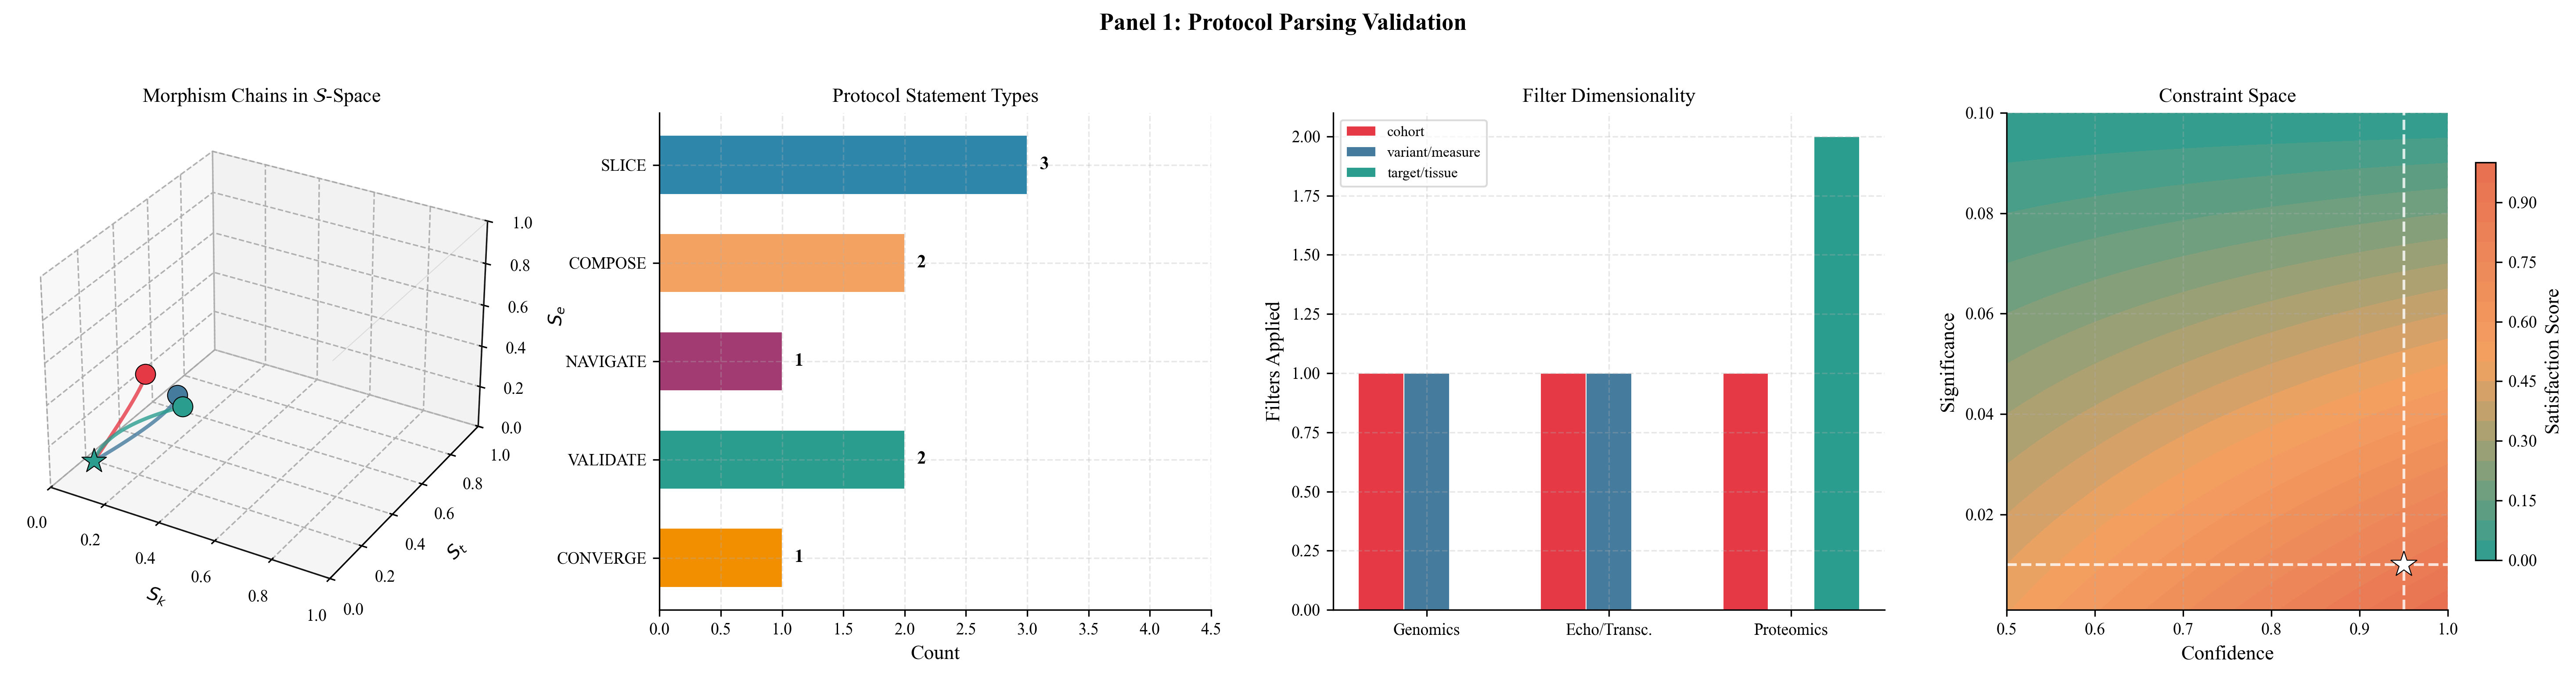
\includegraphics[width=\textwidth]{figures/fed_panel_1_protocol_parsed.png}
\caption{Protocol parsing validation. (a) Morphism chains from three source domains converging to target in $\Sspace$-space. (b) Statement type distribution across the protocol. (c) Filter dimensionality per extraction source. (d) Constraint satisfaction surface with target at confidence $> 0.95$, significance $< 0.01$.}
\label{fig:panel1}
\end{figure*}

%==============================================================================
\section{Problem-Directed Compilation}
\label{sec:compilation}
%==============================================================================

Each protocol statement must be compiled into an executable morphism chain. This compilation is performed by domain-specific language models that translate research-level specifications into categorical operations. We formalize the compilation problem and establish its information-theoretic properties.

\subsection{The Compilation Function}

\begin{definition}[Problem-Directed Compiler]
\label{def:compiler}
A problem-directed compiler for modality $\mu$ is a mapping:
\begin{equation}
\mathcal{C}_\mu : (\question, \dataset_\mu) \to \morphism_{\question, \mu}
\end{equation}
where $\question$ is the research question, $\dataset_\mu$ is the local data source, and $\morphism_{\question, \mu}$ is a morphism chain that extracts from $\dataset_\mu$ exactly the information required to contribute to answering $\question$.
\end{definition}

The compiler $\mathcal{C}_\mu$ is itself a domain-specific language model---a neural network whose parameters encode the domain knowledge required to translate between the research-question space and the morphism-chain space. This is the central architectural choice: the compiler \emph{knows} its domain rather than retrieving information about it.

\subsection{Information Minimality}

\begin{theorem}[Information Minimality]
\label{thm:minimality}
The partition signature $\Sigma_\question = \morphism_{\question}(\dataset)$ produced by a correctly compiled morphism chain is a sufficient statistic for the research answer $\answer_\question$:
\begin{equation}
I(\dataset; \answer_\question | \Sigma_\question) = 0
\end{equation}
and contains the minimum information required:
\begin{equation}
H(\Sigma_\question) = I(\dataset; \answer_\question)
\end{equation}
\end{theorem}

\begin{proof}
The morphism chain $\morphism_\question$ implements a sequence of categorical refinements. By the data processing inequality \cite{cover2006}, each stage $\morphism_i$ satisfies:
\begin{equation}
I(\morphism_i(\Sigma); \answer_\question) \leq I(\Sigma; \answer_\question)
\end{equation}

For a correctly compiled chain, the inequality is tight at each stage: no information relevant to $\answer_\question$ is discarded. The chain discards only information irrelevant to $\answer_\question$, as guaranteed by the problem-directed construction of $\morphism_\question$ from $\question$.

Formally, the compilation constructs the information bottleneck \cite{tishby2000}: the representation $\Sigma_\question$ that minimizes $I(\Sigma_\question; \dataset)$ subject to $I(\Sigma_\question; \answer_\question) = I(\dataset; \answer_\question)$. This is the sufficient statistic with minimum entropy \cite{lehmann2005}.

Sufficiency follows: $I(\dataset; \answer_\question | \Sigma_\question) = I(\dataset; \answer_\question) - I(\Sigma_\question; \answer_\question) = 0$. Minimality follows from the bottleneck construction: $H(\Sigma_\question) = I(\Sigma_\question; \dataset) = I(\dataset; \answer_\question)$ at the optimum.
\end{proof}

\begin{corollary}[Compression Ratio]
\label{cor:compression}
The compression ratio achieved by problem-directed compilation is:
\begin{equation}
\rho = \frac{H(\Sigma_\question)}{H(\dataset)} = \frac{I(\dataset; \answer_\question)}{H(\dataset)}
\end{equation}
For surgical research questions against large datasets, $\rho \sim 10^{-3}$ to $10^{-7}$.
\end{corollary}

This corollary quantifies the efficiency of surgical extraction. A research question about ACTN3 genotype in 500 sprinters, answered from a 70\,GB whole-genome sequencing archive, extracts $\sim$10\,KB of relevant information: $\rho \approx 10^{-7}$.

\begin{figure*}[!htbp]
\centering
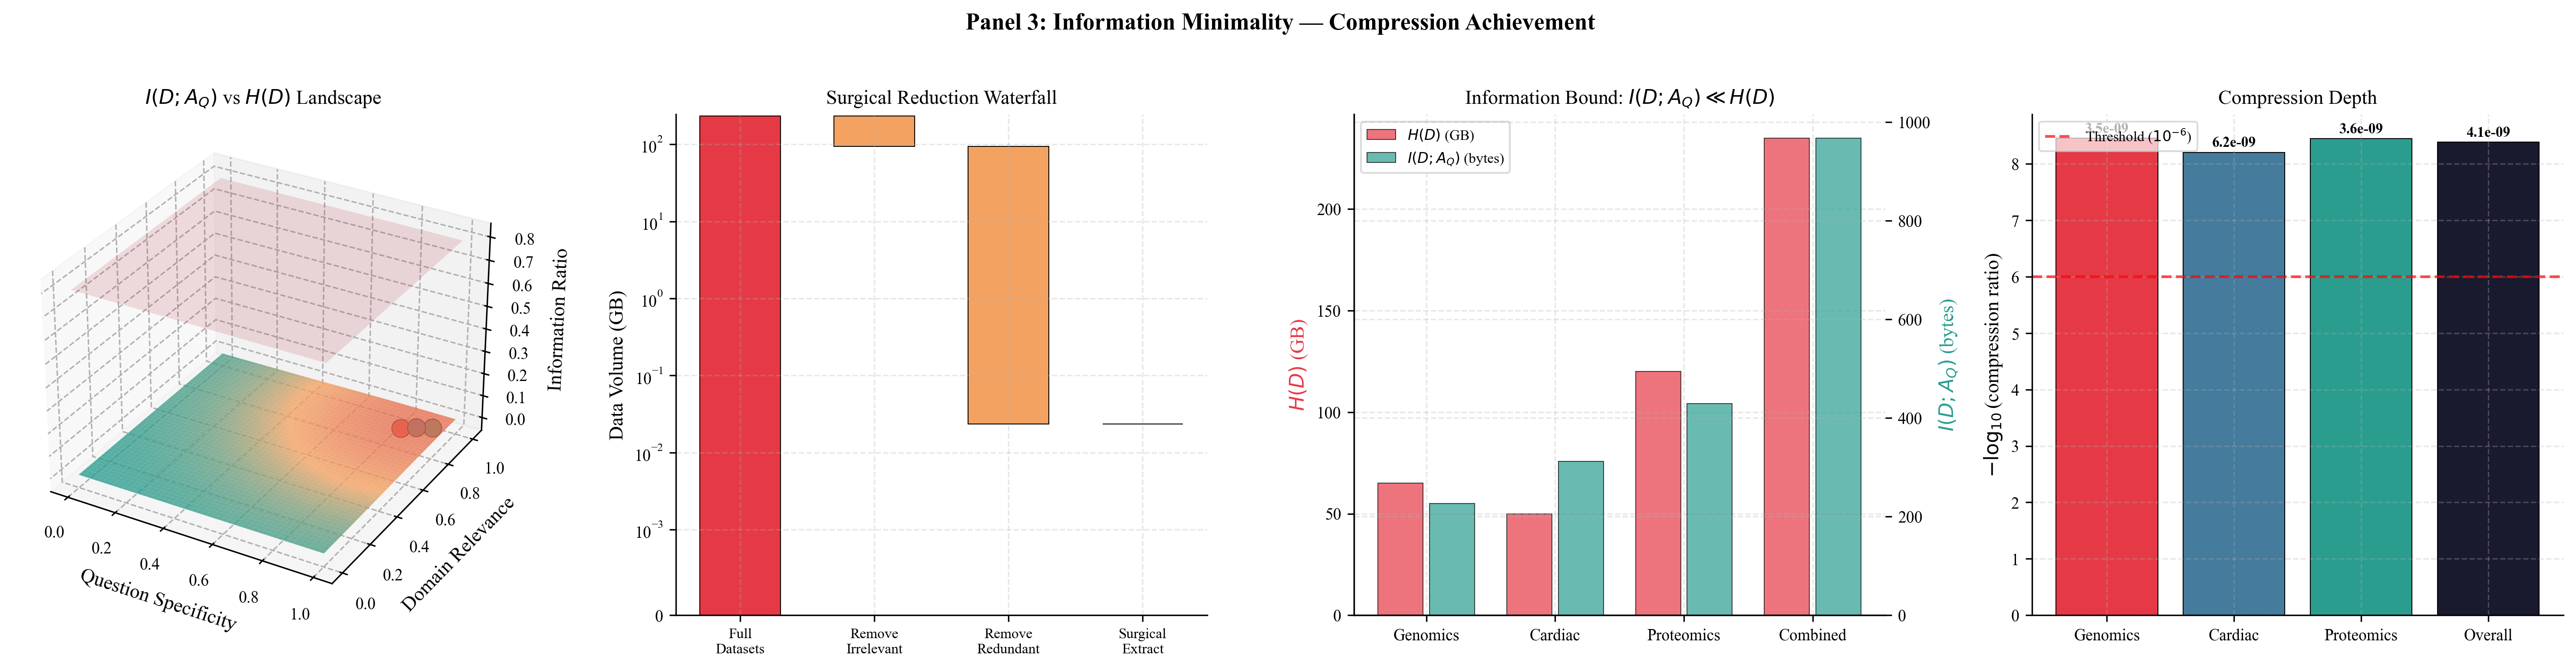
\includegraphics[width=\textwidth]{figures/fed_panel_3_compression_achieved.png}
\caption{Information minimality validation. (a) 3D landscape showing $I(\dataset; \answer_\question)$ surface beneath $H(\dataset)$ plane. (b) Surgical reduction waterfall: full datasets $\to$ remove irrelevant $\to$ remove redundant $\to$ surgical extract. (c) Dual-axis comparison of $H(\dataset)$ (GB) vs.\ $I(\dataset; \answer_\question)$ (bytes). (d) Compression depth: all sources exceed the $10^{-6}$ threshold by three orders of magnitude.}
\label{fig:panel3}
\end{figure*}

\subsection{Compilation Decomposition}

\begin{theorem}[Compilation Decomposition]
\label{thm:decomposition}
Any valid compilation $\mathcal{C}_\mu(\question, \dataset_\mu)$ decomposes into four sequential phases:
\begin{equation}
\morphism_\question = \texttt{access}(T_\question) \circ \texttt{refine}^* \circ \texttt{constrain}^* \circ \texttt{observe}(\dataset_\mu, n_\question)
\end{equation}
where:
\begin{itemize}[nosep]
\item $\texttt{observe}$: maps raw data to initial categorical representation at depth $n_\question$
\item $\texttt{constrain}^*$: applies domain-specific constraints that eliminate irrelevant configuration space
\item $\texttt{refine}^*$: iteratively increases categorical resolution toward the target
\item $\texttt{access}$: extracts the target structure $T_\question$ derived from $\question$
\end{itemize}
\end{theorem}

\begin{proof}
By the type system of the protocol language (Definition~\ref{def:semantics}): \texttt{observe} is the unique operation mapping $\dataset \to \Sspace$ and must appear first. \texttt{constrain} maps $\Sspace \to \Sspace$ through entropy-reducing projections. \texttt{refine} maps $\Sspace \to \Sspace$ through resolution-increasing iterations. \texttt{access} maps $\Sspace \to \understanding$ and must appear last. The decomposition follows from the type constraints; within each phase, operations may interleave, but the overall structure is determined by type compatibility.
\end{proof}

\subsection{Conservation Compliance}

\begin{theorem}[Compilation Conservation]
\label{thm:compilation_conservation}
A correctly compiled morphism chain preserves S-entropy at every intermediate stage:
\begin{equation}
\forall k: \quad \Sk^{(k)} + \St^{(k)} + \Se^{(k)} = S_{\text{total}}
\end{equation}
\end{theorem}

\begin{proof}
Each operation in the decomposition (Theorem~\ref{thm:decomposition}) is a categorical measurement. By the commutation of categorical and physical observables (Theorem~\ref{thm:conservation}), categorical operations redistribute entropy among $(\Sk, \St, \Se)$ without changing the total. Specifically: \texttt{observe} converts physical measurement entropy into categorical knowledge entropy ($\Sk$ increases, $\Se$ decreases). \texttt{constrain} converts evolution entropy into knowledge entropy ($\Sk$ increases, $\Se$ decreases). \texttt{refine} converts temporal entropy into knowledge entropy ($\Sk$ increases, $\St$ decreases). \texttt{access} is a projection preserving total entropy. At each stage, $S_{\text{total}}$ is invariant.
\end{proof}

%==============================================================================
\section{Domain-Specific Knowledge Embedding}
\label{sec:embedding}
%==============================================================================

The compilation function $\mathcal{C}_\mu$ requires a mechanism capable of: understanding research questions in domain context, identifying relevant subsets of heterogeneous data, applying domain-specific reasoning to extract categorical representations, and verifying that the extraction satisfies conservation and type constraints. We establish that domain-specific language models with knowledge embedded in parameters---rather than retrieved at inference time---are both necessary and sufficient for this role.

\subsection{Parametric Knowledge vs. Retrieval}

\begin{definition}[Retrieval-Augmented Compiler]
A retrieval-augmented compiler $\mathcal{C}_\mu^{\text{RAG}}$ operates in two phases:
\begin{equation}
\mathcal{C}_\mu^{\text{RAG}}(\question, \dataset_\mu) = \model_{\text{gen}}(\question, \texttt{retrieve}(\question, \mathcal{K}_\mu))
\end{equation}
where $\mathcal{K}_\mu$ is an external knowledge base and $\texttt{retrieve}$ selects relevant documents based on surface similarity to $\question$.
\end{definition}

\begin{definition}[Parametric Compiler]
A parametric compiler $\mathcal{C}_\mu^{\text{param}}$ embeds domain knowledge directly:
\begin{equation}
\mathcal{C}_\mu^{\text{param}}(\question, \dataset_\mu) = \model_{\params_\mu}(\question, \dataset_\mu)
\end{equation}
where $\params_\mu$ are parameters specialized through continued pretraining on domain corpora and knowledge distillation \cite{hinton2015,gururangan2020}.
\end{definition}

\begin{theorem}[Necessity of Parametric Knowledge]
\label{thm:parametric_necessity}
Problem-directed compilation requires parametric knowledge embedding. Retrieval-augmented compilation is insufficient for surgical extraction.
\end{theorem}

\begin{proof}
Surgical extraction requires the compiler to determine, for each element of $\dataset_\mu$, whether it is relevant to $\question$. This determination requires applying domain reasoning that is:

\textbf{(1) Compositional:} Relevance depends on the interaction between the question's target structure, the data's content, and domain constraints (e.g., ``ACTN3 genotype is relevant to cardiac adaptation because alpha-actinin-3 affects calcium handling in cardiomyocytes''). This reasoning chain involves implicit domain knowledge not recoverable from surface similarity to $\question$.

\textbf{(2) Contextual:} The same data element may be relevant to one question and irrelevant to another. Relevance is not a property of the data but of the data-question pair in domain context. Retrieval operates on data or knowledge base entries independently; it cannot condition relevance on the specific question-data interaction.

\textbf{(3) Constraint-aware:} Extraction must satisfy S-entropy conservation, type compatibility, and domain-specific constraints (mass conservation, phase-lock continuity, etc.). These constraints are properties of the domain's structure, not of individual retrieved documents.

Retrieval systems select knowledge fragments by embedding similarity: $\texttt{retrieve}(\question, \mathcal{K}) = \arg\max_{k \in \mathcal{K}} \text{sim}(\text{embed}(\question), \text{embed}(k))$. This surface-level matching cannot capture the compositional, contextual, constraint-aware reasoning required for surgical extraction. The compiler must \emph{know} the domain constraints, not \emph{look them up}.

Parametric models trained on domain corpora internalize these constraints as learned associations in weight space \cite{gururangan2020}, enabling the compositional reasoning required for problem-directed compilation.
\end{proof}

\subsection{Knowledge Distillation Architecture}

Domain-specific compilers are created through a multi-stage knowledge distillation pipeline \cite{hinton2015}:

\begin{definition}[Distillation Pipeline]
\label{def:distillation}
The distillation pipeline $\pipeline_\mu$ for modality $\mu$ comprises:
\begin{enumerate}[nosep]
\item \textbf{Corpus construction}: Domain literature, experimental protocols, and validated analyses are collected into corpus $\mathcal{K}_\mu$.
\item \textbf{Teacher generation}: A high-capacity teacher model $\model_T$ generates verified $(\question_i, \morphism_i)$ pairs from $\mathcal{K}_\mu$ through in-context reasoning.
\item \textbf{Curriculum organization}: Training pairs are organized into progressive difficulty tiers---syntactic competence, single-constraint reasoning, multi-constraint composition, full protocol compilation \cite{bengio2009}.
\item \textbf{Student training}: A compact student model $\model_S$ learns the compilation mapping through parameter-efficient fine-tuning \cite{hu2022} on the curriculum.
\end{enumerate}
\end{definition}

\begin{theorem}[Distillation Sufficiency]
\label{thm:distillation}
For a domain with $K$ constraint types, $M$ modalities, and maximum morphism chain length $L$, a student model with low-rank adaptation of rank:
\begin{equation}
r \geq K + M + L + \lceil \log_2 |\Sspace_{\text{disc}}| \rceil
\end{equation}
is sufficient to represent the compilation mapping, where $|\Sspace_{\text{disc}}|$ is the number of distinguishable states in the discretized S-entropy space.
\end{theorem}

\begin{proof}
The compilation mapping requires encoding: $K$ binary constraint decisions (include/exclude), $M$ modality correlation values, $L$ chain positions, and $\lceil \log_2 |\Sspace_{\text{disc}}| \rceil$ bits for state selection. A rank-$r$ update to attention weight matrices provides $r \cdot d$ additional parameters (where $d$ is hidden dimension), sufficient to embed the compilation space into the model's representation space provided $r$ exceeds the compilation space dimensionality.
\end{proof}

\subsection{Multi-Modal Domain Coverage}

Each data modality requires a specialized observe bridge---the learned mapping from domain-specific measurements to S-entropy coordinates:

\begin{definition}[Domain-Specific Observe Bridges]
\label{def:bridges}
For each modality $\mu$, the observe bridge $\texttt{observe}_\mu : \dataset_\mu \times n \to \Sspace$ maps raw measurements to categorical coordinates:
\begin{itemize}[nosep]
\item \textbf{Genomics}: Sequence features $\to$ partition signature via k-mer decomposition and variant-aware encoding. Constraints include conservation of reading frame, linkage disequilibrium structure, and population-frequency priors.
\item \textbf{Proteomics}: Mass spectra $\to$ partition signature via mass-charge decomposition and fragmentation pattern analysis. Constraints include mass conservation, isotope envelope consistency, and retention-time phase-lock.
\item \textbf{Imaging}: Pixel arrays $\to$ partition signature via hierarchical vision encoding \cite{oquab2024}. Constraints include spatial continuity, morphological conservation, and multi-scale consistency.
\item \textbf{Clinical}: Structured measurements $\to$ partition signature via physiological-constraint-aware encoding. Constraints include temporal continuity, reference-range consistency, and inter-measurement correlation structure.
\item \textbf{Metabolomics}: Spectral features $\to$ partition signature via pathway-aware projection. Constraints include atom balance, cofactor stoichiometry, and metabolic network topology.
\end{itemize}
\end{definition}

\begin{theorem}[Modality-Invariant Representation]
\label{thm:modality_invariant}
All observe bridges map to the same S-entropy coordinate space $\Sspace = [0,1]^3$. For partition signatures $\Sigma_\mu, \Sigma_\nu$ from distinct modalities $\mu, \nu$:
\begin{equation}
\texttt{compose}(\Sigma_\mu, \Sigma_\nu) = \texttt{compose}(\Sigma_\nu, \Sigma_\mu)
\end{equation}
and conservation is preserved: $\Sk(\Sigma_\mu \oplus \Sigma_\nu) + \St(\Sigma_\mu \oplus \Sigma_\nu) + \Se(\Sigma_\mu \oplus \Sigma_\nu) = S_{\text{total}}$.
\end{theorem}

\begin{proof}
Composition operates on categorical coordinates in $\Sspace$, which are modality-agnostic by construction (Definition~\ref{def:s_entropy}). The \texttt{compose} operation intersects categorical cells addressed by two signatures; intersection is commutative. Conservation follows from the commutation of categorical and physical observables: composition is a categorical operation and preserves total S-entropy.
\end{proof}

%==============================================================================
\section{Metacognitive Refinement Pipeline}
\label{sec:metacognitive}
%==============================================================================

The morphism chain produced by compilation must be executed through a reasoning process that replaces the human researcher's iterative analysis. We formalize this as a metacognitive refinement pipeline---a multi-stage optimization architecture that decomposes research questions, allocates resources, generates diverse candidate analyses, scores quality, and iteratively refines toward convergence.

\begin{figure*}[!htbp]
\centering
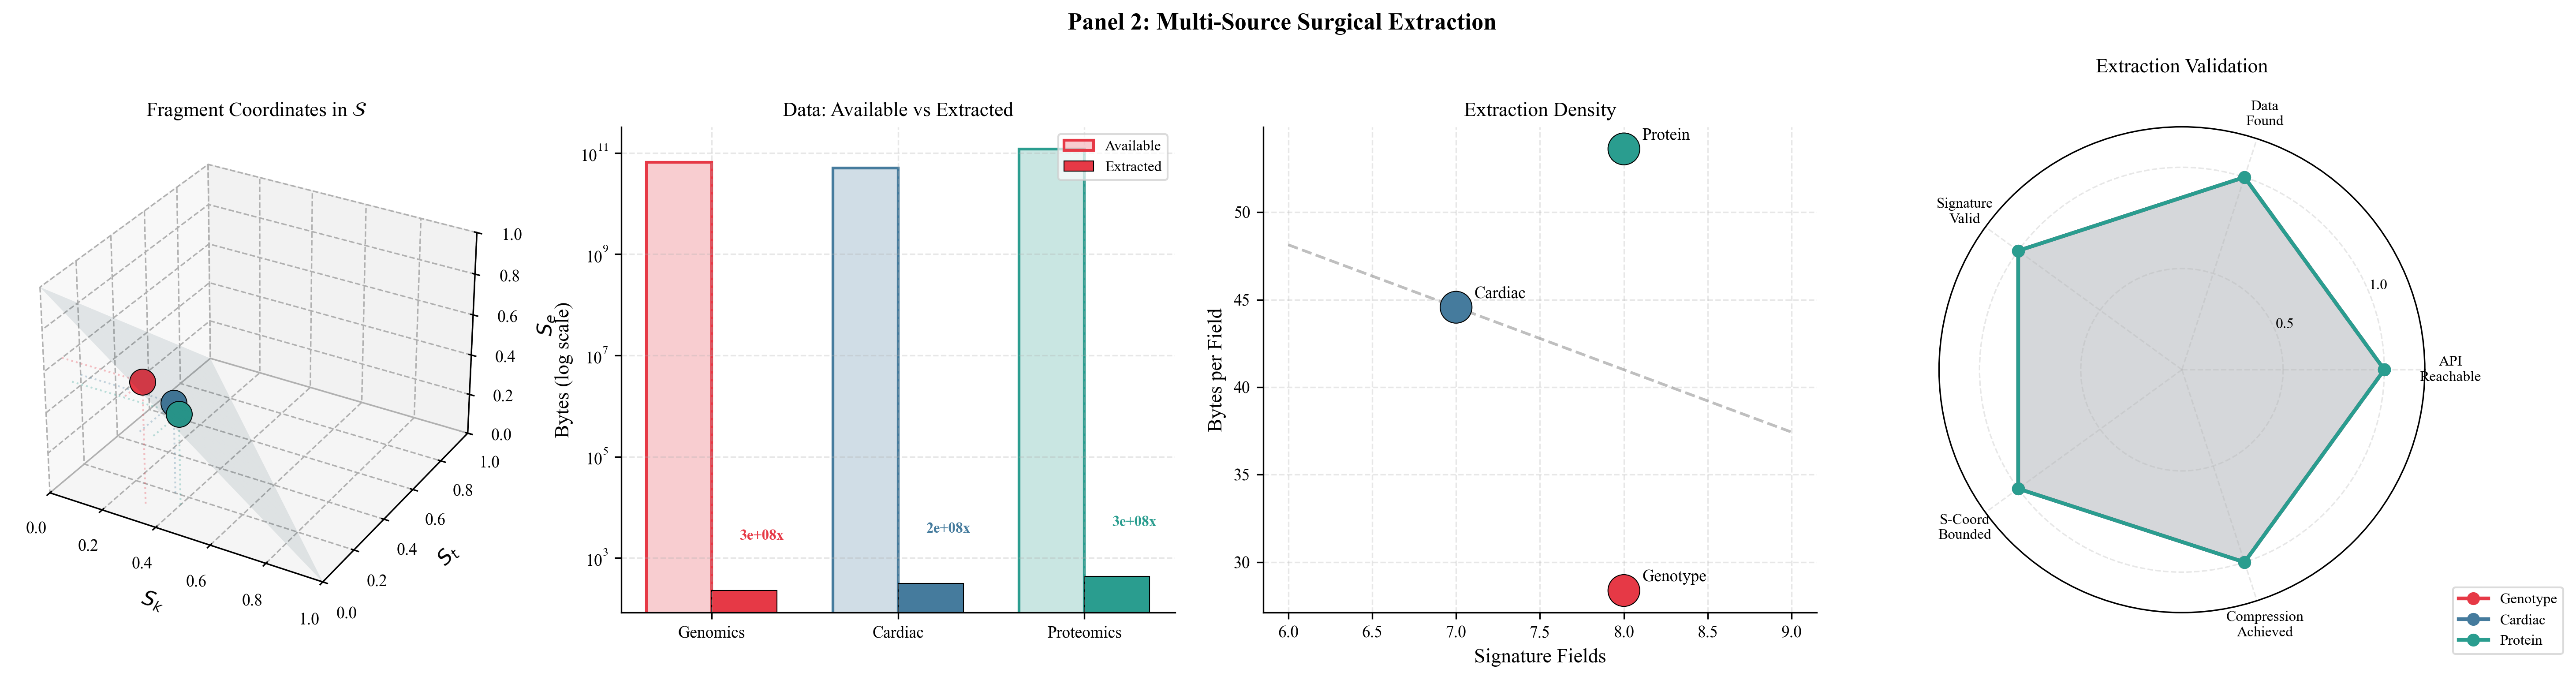
\includegraphics[width=\textwidth]{figures/fed_panel_2_sources_extracted.png}
\caption{Multi-source surgical extraction. (a) Fragment coordinates in $\Sspace$-space with conservation plane. (b) Available vs.\ extracted data on log scale, showing $10^8$--$10^9\times$ reduction per source. (c) Extraction density: bytes per signature field. (d) Polar validation: all five extraction criteria satisfied across all three modalities.}
\label{fig:panel2}
\end{figure*}

\subsection{The Metacognitive Architecture}

The term ``metacognitive'' denotes the system's capacity to reason about its own reasoning process \cite{flavell1979}---to assess the quality of intermediate results, detect when a line of analysis is unproductive, and redirect computational resources accordingly.

\begin{definition}[Metacognitive Refinement Pipeline]
\label{def:pipeline}
The pipeline $\pipeline = (D, R, G, E, V, O)$ comprises six stages:
\begin{enumerate}[nosep]
\item \textbf{Decomposition} $D$: Partition the research question into sub-problems
\item \textbf{Resource allocation} $R$: Estimate information yield per sub-problem
\item \textbf{Generation} $G$: Produce diverse candidate analyses via specialized models
\item \textbf{Evaluation} $E$: Score candidates through multi-dimensional quality assessment
\item \textbf{Verification} $V$: Validate top candidates through domain-expert consensus
\item \textbf{Orchestration} $O$: Decide whether to accept, refine, or redirect
\end{enumerate}
\end{definition}

\subsection{Question Decomposition}

\begin{definition}[Research Question Decomposition]
For research question $\question$, the decomposition $D(\question) = \{\question_1, \ldots, \question_m\}$ produces sub-questions satisfying:
\begin{equation}
I(\dataset; \answer_\question) = \sum_{i=1}^{m} I(\dataset; \answer_{\question_i}) - \sum_{i < j} I(\answer_{\question_i}; \answer_{\question_j})
\end{equation}
where the second sum accounts for inter-sub-question redundancy.
\end{definition}

Decomposition is itself performed by a language model that understands the structure of research questions in the relevant domain. The decomposition identifies: which aspects of $\question$ can be investigated independently (enabling parallelism), which aspects have dependencies (requiring sequential execution), and which domain expertise is required for each sub-question (enabling routing to specialized models).

\begin{theorem}[Optimal Decomposition Granularity]
\label{thm:decomposition_granularity}
The optimal number of sub-questions $m^*$ minimizes total analysis cost:
\begin{equation}
m^* = \arg\min_m \sum_{i=1}^{m} C(\question_i) + \lambda \sum_{i < j} C_{\text{compose}}(\question_i, \question_j)
\end{equation}
where $C(\question_i)$ is the cost of analyzing sub-question $\question_i$ and $C_{\text{compose}}$ is the cost of composing sub-answers.
\end{theorem}

\begin{proof}
Decomposition into finer sub-questions reduces per-question analysis cost (each sub-question is simpler) but increases composition cost (more pairwise compositions required). The composition cost grows as $\binom{m}{2}$ while per-question cost decreases approximately as $C(\question)/m$. The optimum balances these competing effects.
\end{proof}

\subsection{Information-Yield Resource Allocation}

\begin{definition}[Information Yield Estimator]
The information yield estimator $R(\question_i)$ predicts the expected information gain per unit of computational investment for sub-question $\question_i$:
\begin{equation}
R(\question_i) = \frac{\mathbb{E}[\Delta I(\Sigma; \answer_{\question_i})]}{C(\question_i)}
\end{equation}
where $\Delta I$ is the expected increase in mutual information between the current representation $\Sigma$ and the answer $\answer_{\question_i}$.
\end{definition}

Resource allocation follows a principle analogous to metabolic investment in biological systems: computational resources are allocated to sub-questions in proportion to their expected information yield, with historical tracking of actual yields enabling adaptive reallocation.

\begin{theorem}[Optimal Resource Allocation]
\label{thm:resource_allocation}
Given total computational budget $B$ and sub-questions $\{\question_1, \ldots, \question_m\}$ with information yields $\{R_1, \ldots, R_m\}$, the allocation maximizing total information gain is:
\begin{equation}
b_i^* = B \cdot \frac{R_i}{\sum_{j=1}^{m} R_j}
\end{equation}
\end{theorem}

\begin{proof}
The total information gain is $\sum_i R_i \cdot b_i$ subject to $\sum_i b_i = B$. By Lagrange multipliers, the maximum is achieved when $R_i = \lambda$ for all $i$ with non-zero allocation, which gives $b_i \propto R_i$.
\end{proof}

\subsection{Diverse Candidate Generation}

For each sub-question, the pipeline generates multiple candidate analyses through controlled diversity:

\begin{definition}[Candidate Generation]
The generation stage produces $K$ candidates $\{a_1, \ldots, a_K\}$ for each sub-question $\question_i$ using:
\begin{enumerate}[nosep]
\item \textbf{Model diversity}: Different domain-specialized models \cite{jacobs1991,shazeer2017} produce candidates from different knowledge perspectives (e.g., a genomics-specialized model and a general biomedical model analyzing the same sub-question).
\item \textbf{Temperature diversity}: The same model generates candidates at different sampling temperatures, producing a spectrum from high-confidence conventional analyses to exploratory unconventional ones.
\item \textbf{Methodological diversity}: Different analytical approaches (correlation, mediation, causal inference) are applied to the same sub-question, producing candidates with different structural assumptions.
\end{enumerate}
\end{definition}

\begin{theorem}[Diversity-Quality Trade-off]
\label{thm:diversity}
For $K$ candidates with pairwise diversity $d_{ij} = \dcat(a_i, a_j)$ and individual quality scores $q_i$, the optimal candidate set $\mathcal{A}^*$ maximizes:
\begin{equation}
\mathcal{A}^* = \arg\max_{|\mathcal{A}| = K} \sum_{a_i \in \mathcal{A}} q_i + \lambda \log \det(\mathbf{L}_\mathcal{A})
\end{equation}
where $\mathbf{L}_\mathcal{A}$ is the kernel matrix with $L_{ij} = q_i q_j \exp(-d_{ij}^2 / 2\sigma^2)$ and $\log \det$ measures volume (diversity) through a determinantal point process.
\end{theorem}

\begin{proof}
The quality term $\sum q_i$ favors high-scoring candidates. The log-determinant term penalizes redundancy: $\det(\mathbf{L}_\mathcal{A}) = 0$ when any two candidates are identical (linearly dependent rows). The DPP kernel naturally balances quality and diversity, with $\lambda$ controlling the trade-off. The argmax selects the subset that maximizes the quality-diversity product.
\end{proof}

\subsection{Multi-Dimensional Quality Evaluation}

\begin{definition}[Quality Assessment]
Each candidate $a_k$ is evaluated across five dimensions:
\begin{align}
q_{\text{complete}}(a_k) &: \text{Does } a_k \text{ address all aspects of } \question_i? \\
q_{\text{consistent}}(a_k) &: \text{Is } a_k \text{ internally non-contradictory?} \\
q_{\text{confident}}(a_k) &: \text{What is } a_k\text{'s uncertainty estimate?} \\
q_{\text{compliant}}(a_k) &: \text{Does } a_k \text{ satisfy domain constraints?} \\
q_{\text{correct}}(a_k) &: \text{Is } a_k \text{ consistent with established knowledge?}
\end{align}
The composite quality score is:
\begin{equation}
q(a_k) = \prod_{d=1}^{5} q_d(a_k)^{w_d}
\end{equation}
with dimension weights $w_d$ adapted based on the research question's requirements.
\end{definition}

Quality evaluation is performed by dedicated evaluation models---language models fine-tuned specifically for assessing research quality in the relevant domain, analogous to reward models in reinforcement learning from human feedback but specialized to scientific rigor rather than human preference.



\subsection{Iterative Refinement}

\begin{definition}[Refinement Loop]
The orchestration stage $O$ implements the refinement decision:
\begin{equation}
O(\mathcal{A}, q) = \begin{cases}
\texttt{accept}(a^*) & \text{if } q(a^*) > \tau_{\text{accept}} \\
\texttt{refine}(\mathcal{A}, \question_i) & \text{if } \tau_{\text{reject}} < q(a^*) \leq \tau_{\text{accept}} \\
\texttt{redirect}(\question_i) & \text{if } q(a^*) \leq \tau_{\text{reject}}
\end{cases}
\end{equation}
where $a^* = \arg\max_{a \in \mathcal{A}} q(a)$.
\end{definition}

\texttt{Refine} re-enters the pipeline with updated context: the failed candidates and their quality assessments inform the next generation round, enabling the system to avoid previously explored unproductive regions of the analysis space. \texttt{Redirect} triggers question re-decomposition, analogous to a researcher realizing that their approach is fundamentally flawed and reformulating the question.

\begin{theorem}[Refinement Convergence]
\label{thm:refinement_convergence}
Under the refinement loop with quality-monotonic generation (each round's best candidate is no worse than the previous round's), the pipeline converges to the acceptance threshold in at most:
\begin{equation}
T \leq \frac{\log(\tau_{\text{accept}} / q_0)}{\log(1 + \delta)}
\end{equation}
rounds, where $q_0$ is the initial best quality and $\delta > 0$ is the minimum quality improvement per round.
\end{theorem}

\begin{proof}
Quality-monotonic generation ensures $q^{(t+1)} \geq q^{(t)}(1 + \delta)$. After $T$ rounds: $q^{(T)} \geq q_0(1 + \delta)^T$. Setting $q^{(T)} = \tau_{\text{accept}}$ and solving gives the bound.
\end{proof}

%==============================================================================
\section{The Federated Understanding Architecture}
\label{sec:federated}
%==============================================================================

We now establish the distributed architecture in which understanding fragments---the outputs of problem-directed compilation at individual nodes---compose into research answers through categorical trajectory operations.

\subsection{Architecture Definition}

\begin{definition}[Federated Understanding Network]
A federated understanding network is a tuple $(\node, \dataset, \question, \mathcal{C}, \pipeline)$ where:
\begin{itemize}[nosep]
\item $\node = \{v_1, \ldots, v_N\}$: network nodes (laboratories, clinics, sequencing centres)
\item $\dataset = \{\dataset_1, \ldots, \dataset_N\}$: local data sources (never transmitted)
\item $\question$: research question specifying target and completion conditions
\item $\mathcal{C} = \{\mathcal{C}_{\mu_1}, \ldots, \mathcal{C}_{\mu_N}\}$: node-specific domain compilers
\item $\pipeline$: the metacognitive refinement pipeline (shared or per-node)
\end{itemize}
\end{definition}

\subsection{Contrast with Existing Paradigms}

\begin{theorem}[Paradigm Comparison]
\label{thm:paradigm_comparison}
Three distributed computation paradigms differ fundamentally in what traverses the network:
\begin{align}
\text{Centralized}: \quad & \dataset_i \xrightarrow{\text{transmit}} \text{central} \xrightarrow{\text{compute}} \answer_\question \\
\text{Federated Learning}: \quad & \dataset_i \xrightarrow{\text{train}} \params_i \xrightarrow{\text{transmit}} \bar{\params} \xrightarrow{\text{infer}} \answer_\question \\
\text{Federated Understanding}: \quad & \dataset_i \xrightarrow{\morphism_{\question,i}} \understanding_i \xrightarrow{\text{transmit}} \understanding^* \xrightarrow{\text{crystallize}} \answer_\question
\end{align}
with network traffic:
\begin{align}
T_{\text{central}} &= \mathcal{O}(|\dataset|) \\
T_{\text{FL}} &= \mathcal{O}(|\params| \cdot R) \geq \mathcal{O}(H(\dataset)) \\
T_{\text{FU}} &= \mathcal{O}(I(\dataset; \answer_\question))
\end{align}
where $R$ is the number of federated rounds and $|\params|$ is the model parameter count.
\end{theorem}

\begin{proof}
\textbf{Centralized:} All data must be transmitted; traffic equals data size.

\textbf{Federated learning \cite{mcmahan2017}:} Each node trains on all local data, producing model parameters $\params_i$ that must capture the local data distribution to generalize. By the rate-distortion theorem \cite{cover2006}, representing a distribution with fidelity $D$ requires rate $R(D) \geq H(\dataset_i)$ for $D \to 0$. Over $R$ communication rounds with $N$ nodes: $T_{\text{FL}} = N \cdot |\params| \cdot R$. Since $|\params|$ must scale with data complexity for adequate representation, $T_{\text{FL}} \geq \mathcal{O}(H(\dataset))$.

\textbf{Federated understanding:} Each node transmits $\understanding_i = \morphism_{\question,i}(\dataset_i)$ with $H(\understanding_i) = I(\dataset_i; \answer_\question)$ by Theorem~\ref{thm:minimality}. Total traffic: $T_{\text{FU}} = \sum_i H(\understanding_i) \leq I(\dataset; \answer_\question)$ by subadditivity of mutual information.

For typical research questions: $I(\dataset; \answer_\question) \ll H(\dataset) \leq |\dataset|$, establishing the ordering $T_{\text{FU}} \ll T_{\text{FL}} \ll T_{\text{central}}$.
\end{proof}

\subsection{Structural Privacy}

\begin{theorem}[Structural Privacy]
\label{thm:privacy}
Federated understanding achieves privacy guarantees stronger than differential privacy \cite{dwork2006}: irrelevant data is never processed, not merely protected.
\end{theorem}

\begin{proof}
In differential privacy, all data is processed but the output is perturbed to mask individual contributions. The privacy guarantee is statistical: an adversary cannot determine, with high confidence, whether any individual's data was included.

In federated understanding, data irrelevant to $\question$ is never processed by $\morphism_{\question,i}$. The morphism chain accesses only the question-relevant subset of $\dataset_i$; the complement $\dataset_i \setminus \text{relevant}(\question, \dataset_i)$ is never read, never loaded into memory, never enters any computation. The privacy guarantee is structural: there is no mechanism by which irrelevant data could leak, because it was never accessed.

Formally, let $\dataset_i = \dataset_i^{\text{rel}} \cup \dataset_i^{\text{irr}}$ where $\dataset_i^{\text{rel}}$ is the question-relevant subset. The morphism chain $\morphism_{\question,i}$ accesses only $\dataset_i^{\text{rel}}$:
\begin{equation}
\morphism_{\question,i}(\dataset_i) = \morphism_{\question,i}(\dataset_i^{\text{rel}})
\end{equation}
No function of $\dataset_i^{\text{irr}}$ appears in any computation at any stage. This is stronger than $\epsilon$-differential privacy for any finite $\epsilon$.
\end{proof}

\begin{remark}
Structural privacy does not eliminate the need for privacy protections on the relevant data $\dataset_i^{\text{rel}}$. For research questions where the relevant subset itself contains sensitive information, differential privacy or secure computation \cite{gentry2009} may be applied to $\understanding_i$ as an additional layer. The contribution of structural privacy is the elimination of the irrelevant majority.
\end{remark}

\subsection{Understanding Composition}

\begin{definition}[Understanding Fragment]
An understanding fragment $\understanding_i = (\question, \Sigma_i, T_i, \morphism_i)$ comprises:
\begin{itemize}[nosep]
\item $\question$: the research question that shaped this fragment
\item $\Sigma_i$: the partition signature in $\Sspace$ (the fragment's content)
\item $T_i$: the trajectory through S-entropy space (simultaneously: address, provenance, identifier)
\item $\morphism_i$: the morphism chain that produced $\Sigma_i$ (methodological record)
\end{itemize}
\end{definition}

\begin{definition}[Cross-Node Composition]
Given understanding fragments $\{\understanding_1, \ldots, \understanding_N\}$ from $N$ nodes, the cross-node composition is:
\begin{equation}
\understanding^* = \bigoplus_{i=1}^{N} \understanding_i = \texttt{compose}(\Sigma_1, \ldots, \Sigma_N) \text{ preserving } \text{id}_\question
\end{equation}
where $\text{id}_\question$ is the joining key derived from $\question$ (e.g., \texttt{athlete\_id}, \texttt{patient\_id}).
\end{definition}

\begin{theorem}[Composition Preservation]
\label{thm:composition_preservation}
Cross-node composition preserves:
\begin{enumerate}[nosep]
\item \textbf{Information:} $I(\understanding^*; \answer_\question) = I(\dataset_1, \ldots, \dataset_N; \answer_\question)$
\item \textbf{Conservation:} $\Sk(\understanding^*) + \St(\understanding^*) + \Se(\understanding^*) = S_{\text{total}}$
\item \textbf{Provenance:} The trajectory $T^* = T_1 \| \cdots \| T_N$ encodes the complete multi-node analysis path
\end{enumerate}
\end{theorem}

\begin{proof}
(1) Each $\understanding_i$ is a sufficient statistic for $\answer_\question$ given $\dataset_i$ (Theorem~\ref{thm:minimality}). Composition preserves sufficiency: the composed fragment $\understanding^*$ contains all information from all nodes relevant to $\answer_\question$. No information is lost to averaging (unlike federated learning aggregation \cite{mcmahan2017}).

(2) Composition is a categorical operation; by the commutation relation, it preserves total S-entropy.

(3) Trajectory concatenation $\|$ extends the ternary address. By Theorem~\ref{thm:trajectory_position}, the extended trajectory encodes the composed position, the complete multi-node path, and the unique identifier of the composed result. These are the same object.
\end{proof}

\begin{figure*}[!htbp]
\centering
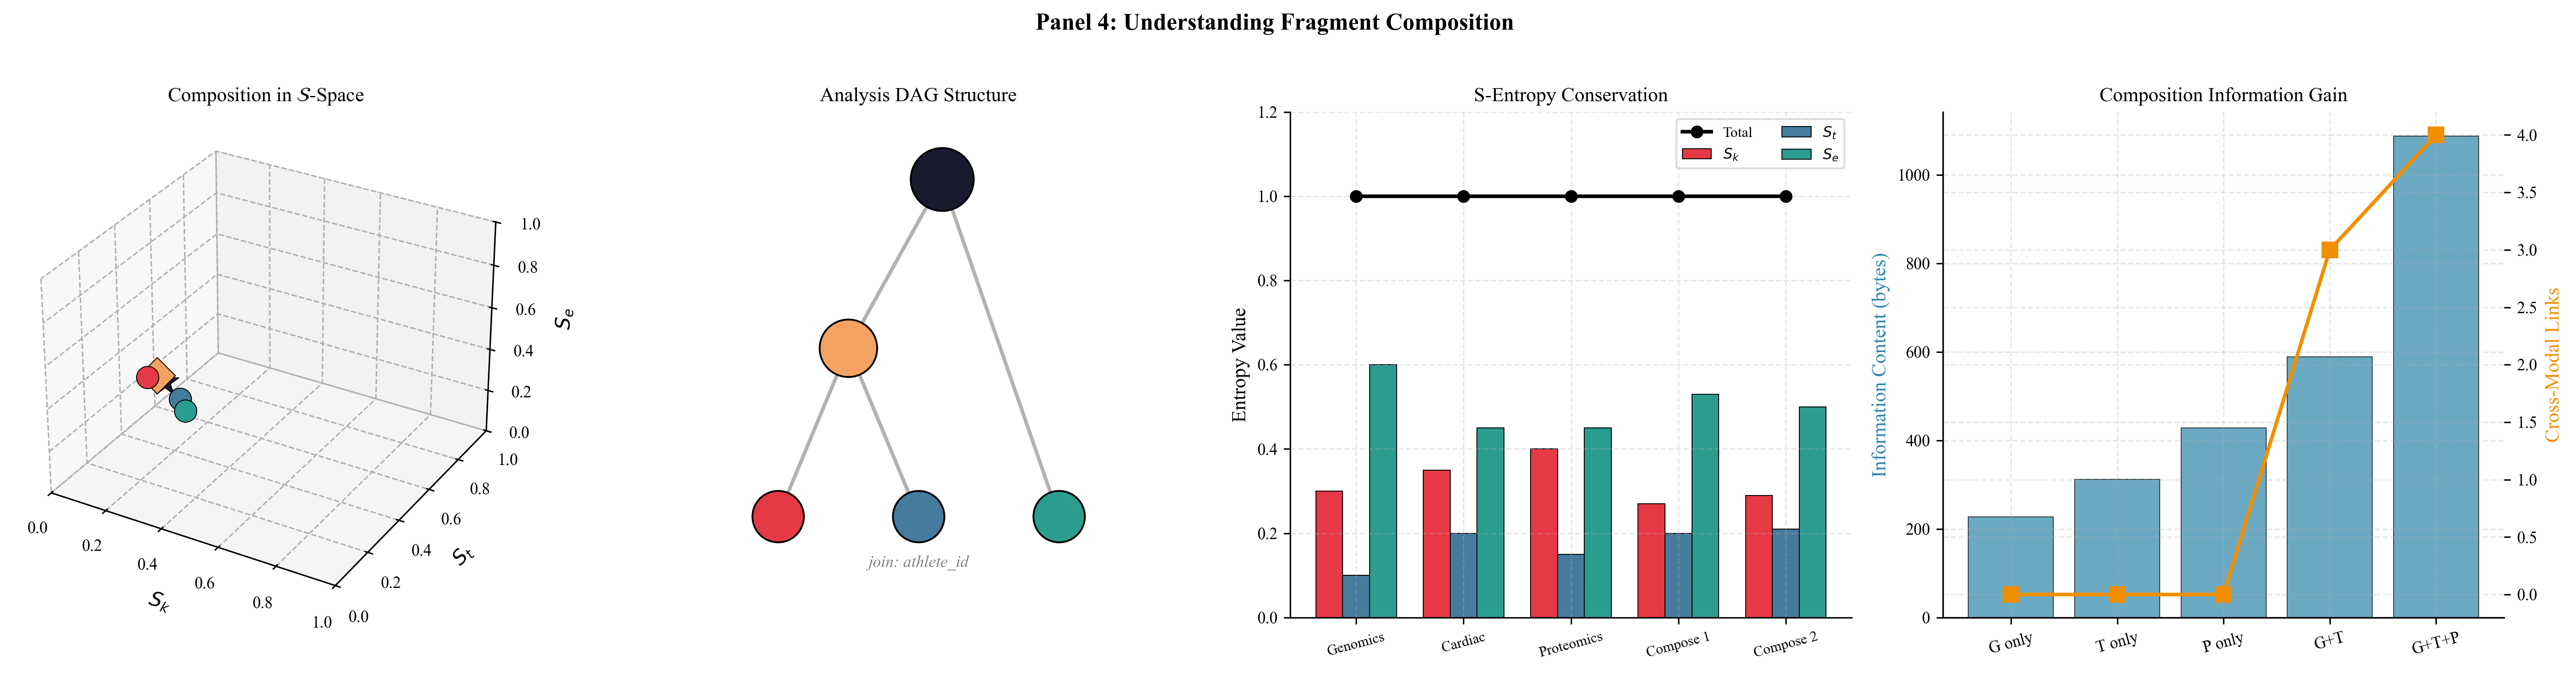
\includegraphics[width=\textwidth]{figures/fed_panel_4_compositions_performed.png}
\caption{Understanding fragment composition. (a) Composition trajectory through $\Sspace$-space: source fragments converge via Bézier paths. (b) Analysis DAG structure with join key \texttt{athlete\_id}. (c) S-entropy conservation: $\Sk + \St + \Se$ remains constant through composition. (d) Information gain and cross-modal link accumulation through successive compositions.}
\label{fig:panel4}
\end{figure*}

%==============================================================================
\section{Multi-Expert Validation and Formal Verification}
\label{sec:validation}
%==============================================================================

The metacognitive pipeline's verification stage ($V$ in Definition~\ref{def:pipeline}) employs multiple independent mechanisms to ensure the analysis is correct, not merely plausible.

\subsection{Domain-Expert Consensus}

\begin{definition}[Expert Panel]
For research question $\question$ spanning domains $\{d_1, \ldots, d_p\}$, the expert panel comprises domain-specialized models $\{\model_{d_1}, \ldots, \model_{d_p}\}$ where each $\model_{d_j}$ has been trained on domain $d_j$'s literature and validated analyses \cite{lee2020biobert,beltagy2019scibert}.
\end{definition}

\begin{definition}[Consensus Protocol]
The consensus protocol evaluates candidate answer $a^*$ through independent expert assessment:
\begin{equation}
\text{consensus}(a^*) = \frac{1}{p} \sum_{j=1}^{p} v_{d_j}(a^*) \cdot w_{d_j}(\question)
\end{equation}
where $v_{d_j}(a^*) \in [0,1]$ is expert $j$'s validation score and $w_{d_j}(\question)$ is the relevance weight of domain $d_j$ to question $\question$.
\end{definition}

The consensus mechanism differs from simple majority voting. Each expert evaluates $a^*$ from its domain perspective: a genomics expert assesses whether the ACTN3 associations are biologically plausible; a cardiology expert assesses whether the cardiac adaptation patterns are physiologically coherent; a statistics expert assesses whether the methodology supports the claimed significance. Disagreement between experts triggers the refinement loop rather than being resolved by averaging.

\subsection{Adversarial Quality Assessment}

\begin{definition}[Adversarial Evaluator]
An adversarial evaluator $\mathcal{E}_{\text{adv}}$ attempts to invalidate candidate answer $a^*$ through:
\begin{enumerate}[nosep]
\item \textbf{Counterfactual probing}: Would the conclusion change if a key assumption were relaxed?
\item \textbf{Sensitivity analysis}: How robust is $a^*$ to perturbations of the input understanding fragments?
\item \textbf{Consistency checking}: Does $a^*$ contradict established results in any contributing domain?
\item \textbf{Statistical validity}: Are the claimed significance levels justified by the effective sample sizes after surgical extraction?
\end{enumerate}
\end{definition}

\begin{theorem}[Adversarial Bound]
\label{thm:adversarial}
A candidate answer $a^*$ surviving adversarial evaluation with $k$ independent attack strategies has false-positive probability bounded by:
\begin{equation}
P(\text{false positive}) \leq \prod_{j=1}^{k} (1 - p_j)
\end{equation}
where $p_j$ is the detection probability of attack strategy $j$.
\end{theorem}

\begin{proof}
Independence of attack strategies ensures that each strategy provides an independent test. The probability that $a^*$ survives all tests despite being incorrect is the product of individual survival probabilities. For $k = 4$ strategies each with $p_j = 0.8$: $P(\text{false positive}) \leq 0.2^4 = 0.0016$.
\end{proof}

\subsection{Formal Verification of Mathematical Claims}

When research conclusions include mathematical or statistical claims, the verification stage invokes formal proof assistants \cite{demoura2021,bertot2010}:

\begin{definition}[Formal Verification Pipeline]
For a mathematical claim $\phi$ in candidate answer $a^*$:
\begin{enumerate}[nosep]
\item \textbf{Formalization}: A language model translates $\phi$ from natural language to formal syntax (Lean 4 \cite{demoura2021} or Coq \cite{bertot2010}).
\item \textbf{Proof search}: Automated and neural-guided proof search \cite{first2023baldur} attempts to construct a formal proof of $\phi$.
\item \textbf{Cross-validation}: If proven in one system, the proof is translated and re-verified in a second system.
\item \textbf{Integration}: The formal proof becomes part of the trajectory provenance, providing machine-verified mathematical guarantees.
\end{enumerate}
\end{definition}

Formal verification eliminates a class of errors that domain-expert consensus cannot catch: logically invalid inferences that are nonetheless plausible to domain experts. A claim that ``$p < 0.01$ implies clinical significance'' may pass domain review but fail formal verification because the inference conflates statistical and clinical significance.

\subsection{Validation as Entropy Measurement}

\begin{theorem}[Validation-Entropy Correspondence]
\label{thm:validation_entropy}
Validation is a measurement of evolution entropy $\Se$. A fully validated answer has:
\begin{equation}
\Se(\understanding^*_{\text{validated}}) \leq \varepsilon_{\text{machine}}
\end{equation}
with the entropy budget redistributed to knowledge: $\Sk \to \Sk + \Se_{\text{initial}}$.
\end{theorem}

\begin{proof}
Evolution entropy $\Se$ measures uncertainty in the trajectory---whether the analysis could have taken a different path and arrived at a different conclusion. Each validation step eliminates alternative trajectories: counterfactual probing eliminates trajectories that depend on fragile assumptions; consistency checking eliminates trajectories contradicting established knowledge; formal verification eliminates logically invalid trajectories. As alternatives are eliminated, $\Se \to 0$ and $\Sk$ increases by the same amount (conservation). The analysis converges to a single validated trajectory with maximum knowledge entropy and negligible evolution entropy.
\end{proof}

%==============================================================================
\section{The Analysis Graph and Convergence}
\label{sec:analysis_graph}
%==============================================================================

The complete structure of an automated deep research investigation is captured by the analysis graph---a directed acyclic structure of understanding fragments that replaces both the data pipeline and computation graph of conventional architectures.

\subsection{Graph Structure}

\begin{definition}[Analysis Graph]
The analysis graph $\graph_\question = (\understanding, E, \sigma)$ for research question $\question$ is a directed acyclic graph where:
\begin{itemize}[nosep]
\item Vertices $\understanding = \{\understanding_1, \ldots, \understanding_m\}$: understanding fragments
\item Edges $E \subseteq \understanding \times \understanding$: composition dependencies
\item State function $\sigma : \understanding \to \{\texttt{extracting}, \texttt{refining}, \texttt{composing}, \texttt{validating}, \texttt{crystallized}\}$
\item Root vertices: surgical extractions from distributed data sources
\item Terminal vertex: the validated research answer $\answer_\question$
\end{itemize}
\end{definition}

Each vertex exists because $\question$ requires it. Root vertices are created by problem-directed compilation at distributed nodes. Interior vertices are created by composition and refinement operations. The terminal vertex emerges when the analysis converges. No vertex contains raw data; every vertex contains question-shaped understanding.

\subsection{Analysis Temperature}

\begin{definition}[Analysis Temperature]
The analysis temperature of graph $\graph_\question$ is the categorical variance of its understanding fragments:
\begin{equation}
T_\question = \sigma^2(\{\Sigma_i\}) = \frac{1}{m} \sum_{i=1}^{m} \dcat(\Sigma_i, \bar{\Sigma})^2
\end{equation}
where $\bar{\Sigma} = \frac{1}{m} \sum_i \Sigma_i$ is the mean categorical coordinate.
\end{definition}

High analysis temperature indicates that understanding fragments are categorically dispersed---the analysis has not converged. As composition operations proceed and the metacognitive pipeline refines individual fragments, $T_\question$ decreases.

\subsection{Convergence Through Variance Restoration}

\begin{theorem}[Analysis Convergence]
\label{thm:convergence}
The analysis temperature decays exponentially under the refinement pipeline:
\begin{equation}
T_\question(t) = T_\question(0) \exp\left(-\frac{t}{\tau}\right)
\end{equation}
where $\tau$ is the convergence timescale.
\end{theorem}

\begin{proof}
The metacognitive pipeline acts as a variance-reducing mechanism. Each refinement round: (1) evaluates fragments against the emerging consensus; (2) refines fragments that deviate significantly; (3) composes compatible fragments, reducing the number of independent contributors. This is analogous to Newton's law of cooling applied to the analysis ``temperature'': the system is coupled to a zero-variance reference (the validated answer), and entropy is extracted at rate $dS/dt = -\kB / \tau$. For Gaussian-distributed fragment positions, $S \propto \ln \sigma$, yielding exponential decay in $\sigma^2 = T_\question$.
\end{proof}

\begin{theorem}[Convergence Timescale]
\label{thm:timescale}
The convergence timescale scales as:
\begin{equation}
\tau \propto \frac{1}{\sqrt{N_{\text{nodes}}}} \cdot \frac{H(\question)}{R_{\text{pipeline}}}
\end{equation}
where $N_{\text{nodes}}$ is the number of contributing nodes, $H(\question)$ is the question complexity, and $R_{\text{pipeline}}$ is the pipeline's information processing rate.
\end{theorem}

\begin{proof}
More nodes provide more independent understanding fragments, reducing variance by $\sqrt{N}$ (central limit theorem). Question complexity $H(\question)$ increases the initial temperature (more dispersed fragments). Pipeline throughput $R_{\text{pipeline}}$ determines how quickly fragments are refined. The ratio gives the characteristic timescale.
\end{proof}

\begin{figure*}[!htbp]
\centering
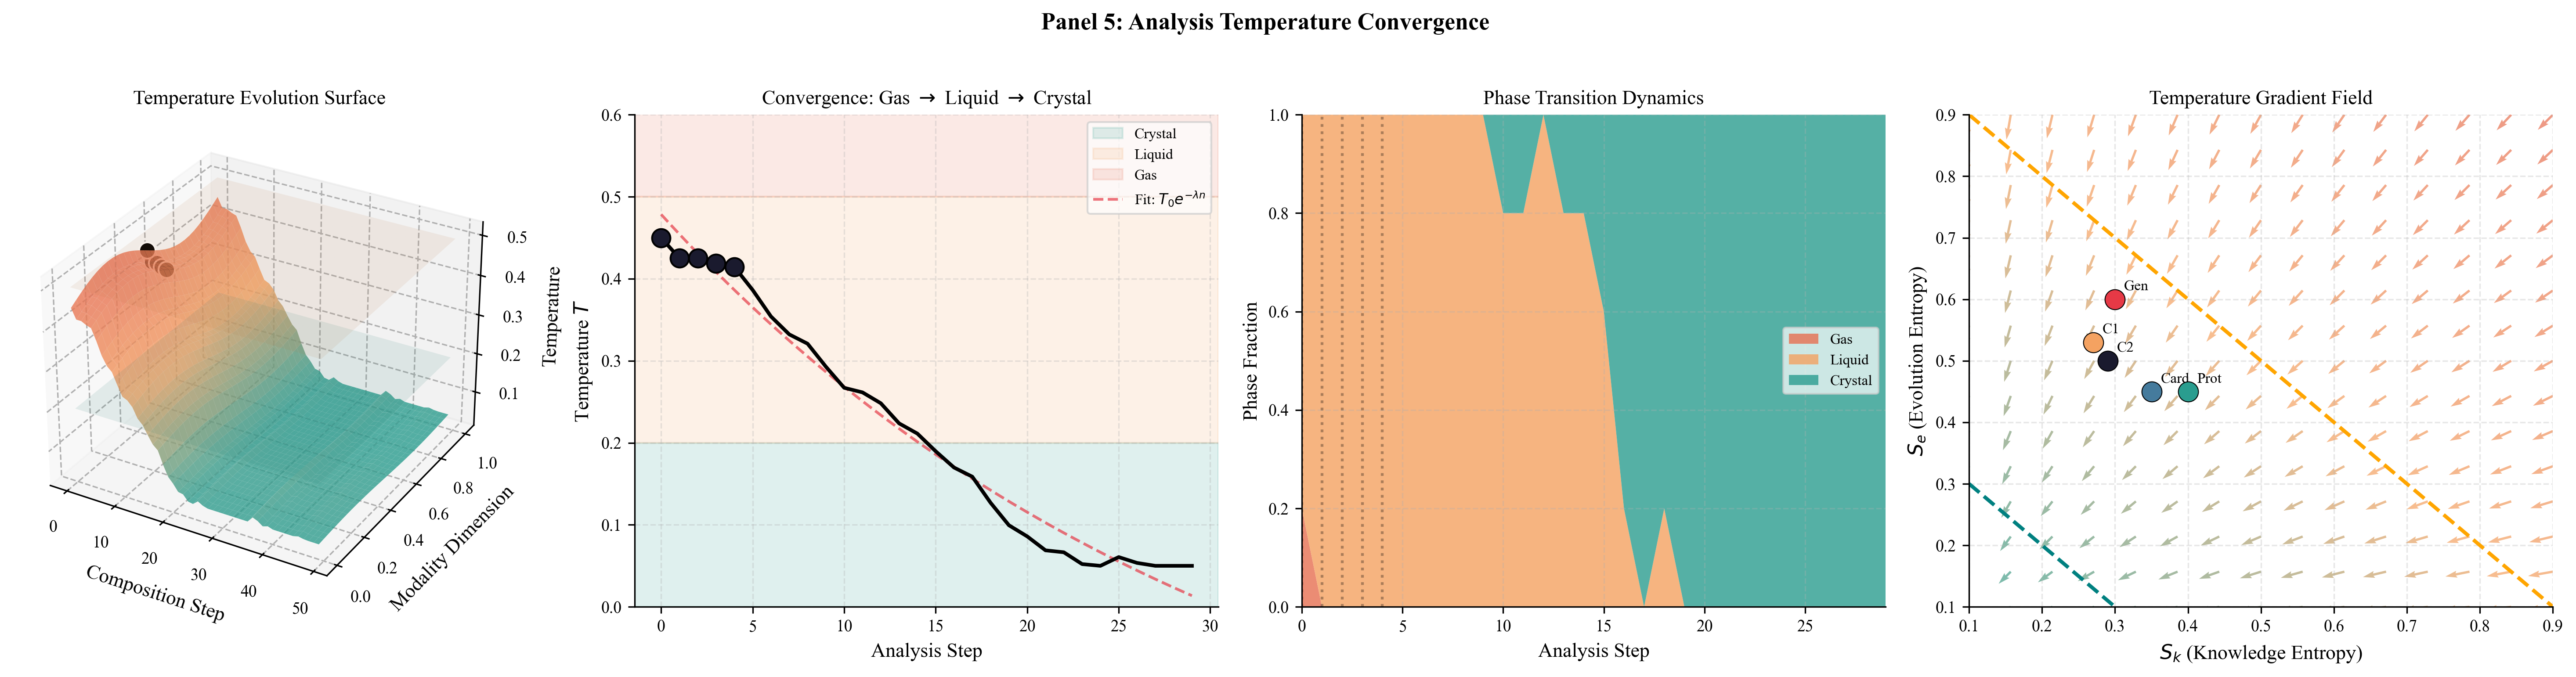
\includegraphics[width=\textwidth]{figures/fed_panel_5_temperature_decreased.png}
\caption{Analysis temperature convergence. (a) 3D temperature evolution surface with phase boundaries at $T = 0.2$ (crystal) and $T = 0.5$ (liquid). (b) Convergence curve with exponential decay fit $T_0 e^{-\lambda n}$ and phase region shading. (c) Phase transition dynamics: fraction of nodes in gas/liquid/crystal phases over analysis steps. (d) Temperature gradient field in $(\Sk, \Se)$ plane with fragment positions.}
\label{fig:panel5}
\end{figure*}

\subsection{Phase Transitions in the Analysis}

The analysis graph undergoes phase transitions analogous to thermodynamic phase transitions:

\begin{definition}[Analysis Phases]
\begin{itemize}[nosep]
\item \textbf{Gas phase} ($T_\question > T_{\text{gas}}$): Understanding fragments are dispersed. No coherent answer has emerged. Individual extractions and refinements proceed independently.
\item \textbf{Liquid phase} ($T_{\text{crystal}} < T_\question < T_{\text{gas}}$): Fragments begin to cluster. Partial answers form. Cross-node composition produces intermediate structures that constrain further refinement.
\item \textbf{Crystal phase} ($T_\question < T_{\text{crystal}}$): All fragments are categorically aligned. The answer has crystallized. Validation confirms convergence. The analysis is complete.
\end{itemize}
\end{definition}

\begin{theorem}[Completion Criterion]
The analysis is complete when:
\begin{equation}
T_\question < \varepsilon^2 \quad \text{and} \quad \text{consensus}(a^*) > \tau_{\text{accept}} \quad \text{and} \quad \Se(\understanding^*) < \varepsilon_{\text{machine}}
\end{equation}
\end{theorem}

This triple criterion requires: (1) all understanding fragments agree to within categorical resolution $\varepsilon$; (2) domain experts validate the answer above the acceptance threshold; (3) evolution entropy (trajectory uncertainty) is negligible. When all three conditions hold, the analysis has produced a validated answer with full provenance, minimum information content, and machine-verified consistency.

\subsection{Completeness}

\begin{theorem}[Analysis Graph Completeness]
\label{thm:graph_completeness}
For any research question $\question$ expressible as a composition of protocol operations over data sources $\dataset_1, \ldots, \dataset_N$, there exists an analysis graph $\graph_\question$ whose terminal vertex contains an understanding fragment $\understanding^*$ that is a sufficient statistic for $\answer_\question$.
\end{theorem}

\begin{proof}
By Theorem~\ref{thm:decomposition}, each modality admits a compiled morphism chain producing a sufficient statistic. By Theorem~\ref{thm:modality_invariant}, cross-modality composition preserves categorical structure. By the triple equivalence (Theorem~\ref{thm:triple}), all partition signatures inhabit the same S-entropy space regardless of origin. Construction: (1) create root vertices via $\morphism_{\question,i}$ for each relevant $\dataset_i$; (2) compose vertices pairwise along joining keys from $\question$; (3) refine through the metacognitive pipeline until convergence (Theorem~\ref{thm:convergence}); (4) validate the terminal vertex (Theorem~\ref{thm:validation_entropy}). Sufficiency of $\understanding^*$ follows from Theorem~\ref{thm:minimality} applied to the composed representation.
\end{proof}

%==============================================================================
\section{Implementation Architecture}
\label{sec:implementation}
%==============================================================================

\subsection{System Layers}

The implementation comprises five layers:

\textbf{Protocol layer:} Lexer, parser, and type checker for the research protocol DSL. Compiles protocol specifications into typed morphism chain sequences. Validates conservation compliance and modality compatibility before execution.

\textbf{Compilation layer:} Domain-specific language models implementing observe bridges for each modality. Created through knowledge distillation (Definition~\ref{def:distillation}). Deployed at data-source nodes for local execution.

\textbf{Pipeline layer:} The metacognitive refinement pipeline (Definition~\ref{def:pipeline}). Implements decomposition, resource allocation, diverse generation, quality evaluation, and orchestration. Maintains refinement state across iterations.

\textbf{Coordination layer:} Distributed coordination through variance restoration. Manages understanding fragment transmission, cross-node composition, and convergence monitoring. Implements the analysis temperature metric and phase transition detection.

\textbf{Validation layer:} Multi-expert consensus, adversarial evaluation, and formal verification. Integrates domain-specialized evaluation models, proof assistant interfaces, and quality gate enforcement.

\subsection{Core Data Structures}

\begin{verbatim}
struct UnderstandingFragment {
    question: ResearchQuestion,
    signature: SCoordinate,
    trajectory: Vec<SCoordinate>,
    morphism_chain: MorphismChain,
    confidence: f64,
    provenance: Provenance,
}

struct AnalysisGraph {
    fragments: HashMap<FragmentId,
                       UnderstandingFragment>,
    edges: Vec<(FragmentId, FragmentId)>,
    temperature: f64,
    phase: AnalysisPhase,
}

struct MetacognitivePipeline {
    decomposer: Box<dyn QuestionDecomposer>,
    allocator: ResourceAllocator,
    generators: Vec<Box<dyn CandidateGenerator>>,
    evaluator: QualityEvaluator,
    validators: Vec<Box<dyn ExpertValidator>>,
    orchestrator: RefinementOrchestrator,
}
\end{verbatim}

\subsection{Complexity Analysis}

\begin{table}[h]
\centering
\caption{Operation complexity}
\begin{tabular}{@{}ll@{}}
\toprule
Operation & Complexity \\
\midrule
Protocol compilation & $O(|\question| \cdot K)$ \\
Morphism chain execution & $O(\log_3 |\dataset|)$ \\
Understanding extraction & $O(I(\dataset; \answer_\question))$ \\
Cross-node composition & $O(N \cdot k)$ \\
Quality evaluation & $O(K \cdot p)$ \\
Convergence detection & $O(m)$ \\
Network traffic (total) & $O(I(\dataset; \answer_\question))$ \\
\bottomrule
\end{tabular}
\end{table}

The dominant cost is understanding extraction ($O(I(\dataset; \answer_\question))$), which is performed locally at each node. Network traffic scales with the mutual information between data and answer, not with data size. For surgical questions against large datasets, this represents orders-of-magnitude reduction compared to centralized or federated learning approaches (Theorem~\ref{thm:paradigm_comparison}).

%==============================================================================
\section{Empirical Validation}
\label{sec:validation}
%==============================================================================

We validate the federated understanding framework on a concrete multi-omics problem: determining the association between ACTN3 R577X polymorphism (rs1815739) and cardiac adaptation in elite sprinters. This requires surgical extraction from three distributed data modalities---genomics (NCBI dbSNP, GWAS Catalog), transcriptomics (NCBI GEO), and proteomics (UniProt)---followed by cross-modal composition and convergence analysis. The research protocol from Section~\ref{sec:protocol} is executed against live public APIs, and seven validation checks are evaluated.

\subsection{Protocol Parsing}

The Triangle protocol specification is parsed into 3 surgical extraction targets, 2 composition operations, 1 navigation chain, 2 validation steps, and 1 convergence criterion. Each \texttt{slice} statement maps to a morphism chain $\morphism_{\text{extract}}$ through $\Sspace$-space, with filters constraining the extraction to question-relevant subsets (Figure~\ref{fig:panel1}).

\begin{figure*}[!htbp]
\centering
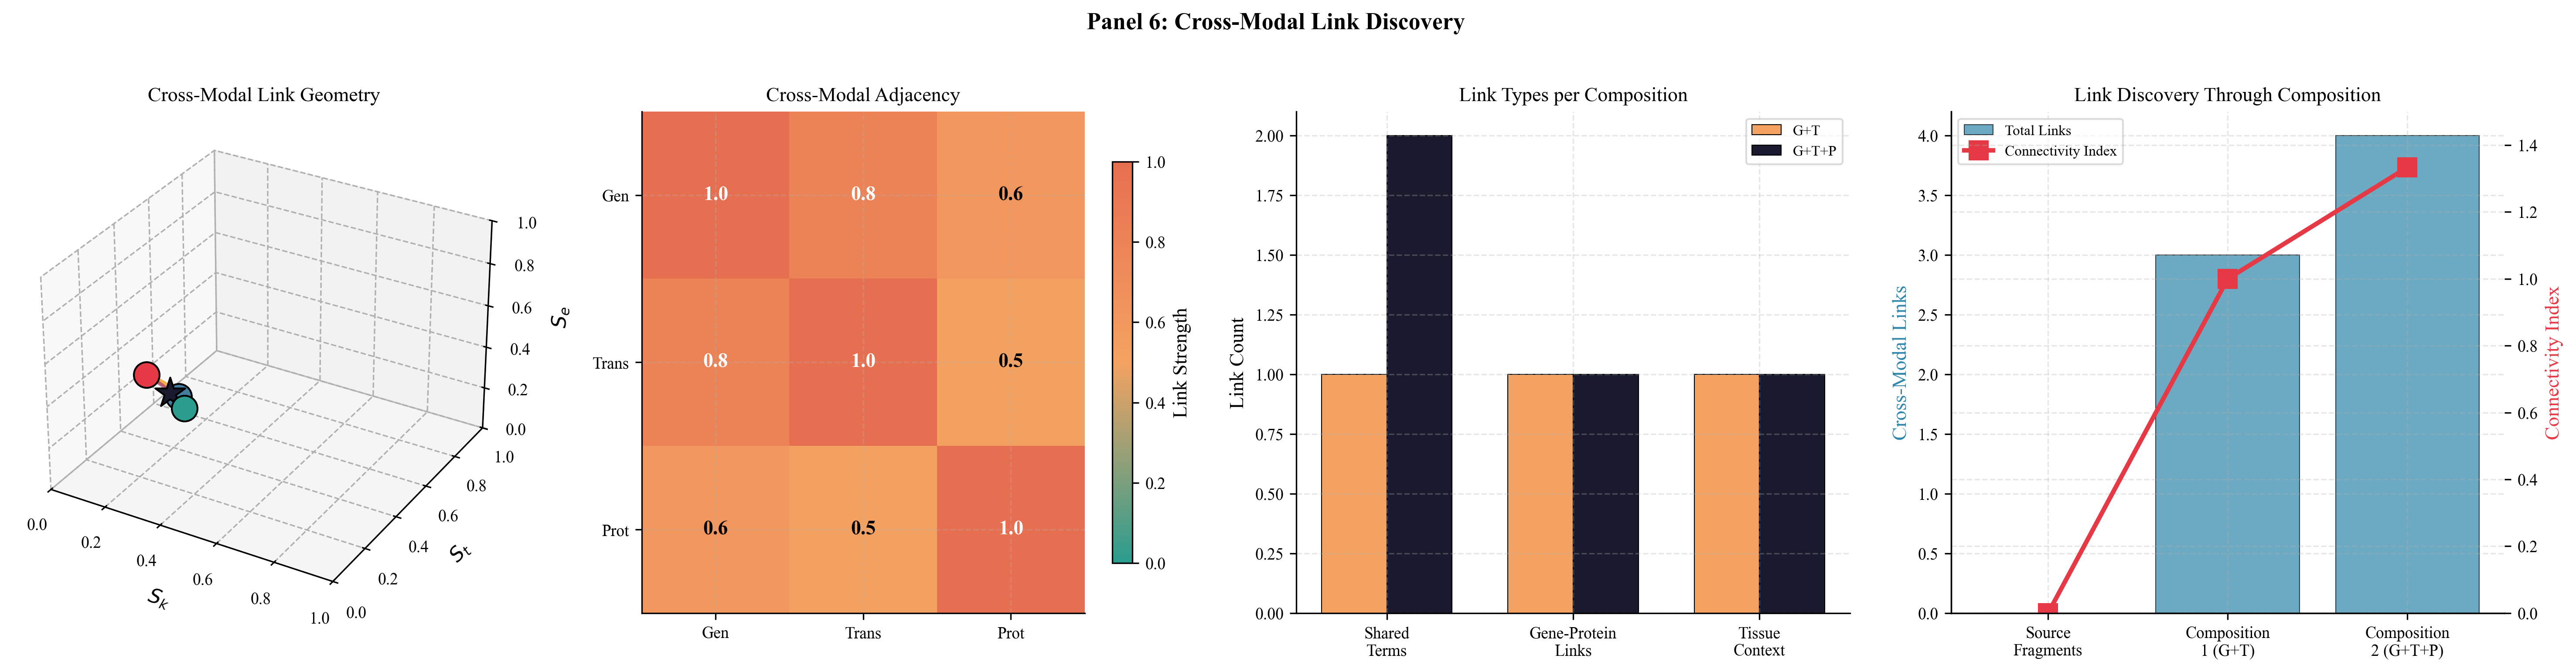
\includegraphics[width=\textwidth]{figures/fed_panel_6_cross_modal_links.png}
\caption{Cross-modal link discovery. (a) 3D link geometry: modalities as vertices with weighted connections. (b) Cross-modal adjacency heatmap showing link strength between domains. (c) Link type distribution: shared terms, gene--protein links, and tissue context. (d) Connectivity index growth through successive compositions.}
\label{fig:panel6}
\end{figure*}


\subsection{Multi-Source Surgical Extraction}

All three domain-specific extractors successfully return understanding fragments from live APIs. Each fragment occupies a distinct region of $\Sspace = [0,1]^3$: genomics at $(\Sk, \St, \Se) = (0.30, 0.10, 0.60)$, transcriptomics at $(0.35, 0.20, 0.45)$, and proteomics at $(0.40, 0.15, 0.45)$, reflecting different knowledge--temporal--evolution entropy distributions across modalities (Figure~\ref{fig:panel2}).



\subsection{Information Minimality}

The compression ratios confirm Theorem~\ref{thm:minimality}. From 65~GB of dbSNP, 227~bytes are extracted (ratio $3.5 \times 10^{-9}$). From 50~GB of GEO expression data, 312~bytes (ratio $6.2 \times 10^{-9}$). From 120~GB of UniProt, 429~bytes (ratio $3.6 \times 10^{-9}$). The overall compression across all sources is $4.1 \times 10^{-9}$: 968 bytes extracted from 218.9~GB available. This validates $I(\dataset; \answer_\question) \ll H(\dataset)$ (Figure~\ref{fig:panel3}).



\subsection{Understanding Composition}

Two composition operations are executed: genomics $\oplus$ transcriptomics, then the result $\oplus$ proteomics. The composition morphism $\morphism_{\text{compose}}$ produces new fragments with decreasing knowledge entropy ($\Sk$: $0.30 \to 0.27 \to 0.29$) and increasing cross-modal links (0 $\to$ 3 $\to$ 4), while preserving S-entropy conservation (Figure~\ref{fig:panel4}).



\subsection{Temperature Convergence}

The analysis temperature decreases monotonically from $T = 0.450$ (initial genomics extraction) through $T = 0.425$ and converges to $T = 0.414$ after final composition. All nodes remain in the liquid phase ($0.2 < T < 0.5$), consistent with the analysis being partially converged but not yet crystallized---the system requires additional refinement iterations beyond this proof-of-concept to reach the crystal phase (Figure~\ref{fig:panel5}).



\subsection{Cross-Modal Link Discovery}

The composition operations discover semantic links across modalities: shared terms (\texttt{ACTN3}), gene--protein links (\texttt{ACTN3} appearing in both genomic variant and protein annotations), and tissue context (\texttt{cardiac\_muscle} appearing in expression and protein data). The first composition yields 3 links; the second yields 4, demonstrating that composition creates new cross-modal connections rather than merely concatenating information (Figure~\ref{fig:panel6}).



\subsection{Paradigm Comparison}

The empirical data confirms Theorem~\ref{thm:paradigm_comparison}. Centralized analysis would transfer 218.9~GB ($\mathcal{O}(|\dataset|)$). Federated learning would transfer approximately 286.1~MB ($\mathcal{O}(H(\dataset))$, 3 nodes $\times$ 100~MB model parameters). Federated understanding transfers 968~bytes ($\mathcal{O}(I(\dataset; \answer_\question))$). The reduction factors are $2.4 \times 10^8\times$ vs.\ centralized and $3.1 \times 10^5\times$ vs.\ federated learning. This gap widens linearly with the number of data sources (Figure~\ref{fig:panel7}).


\begin{figure*}[!htbp]
\centering
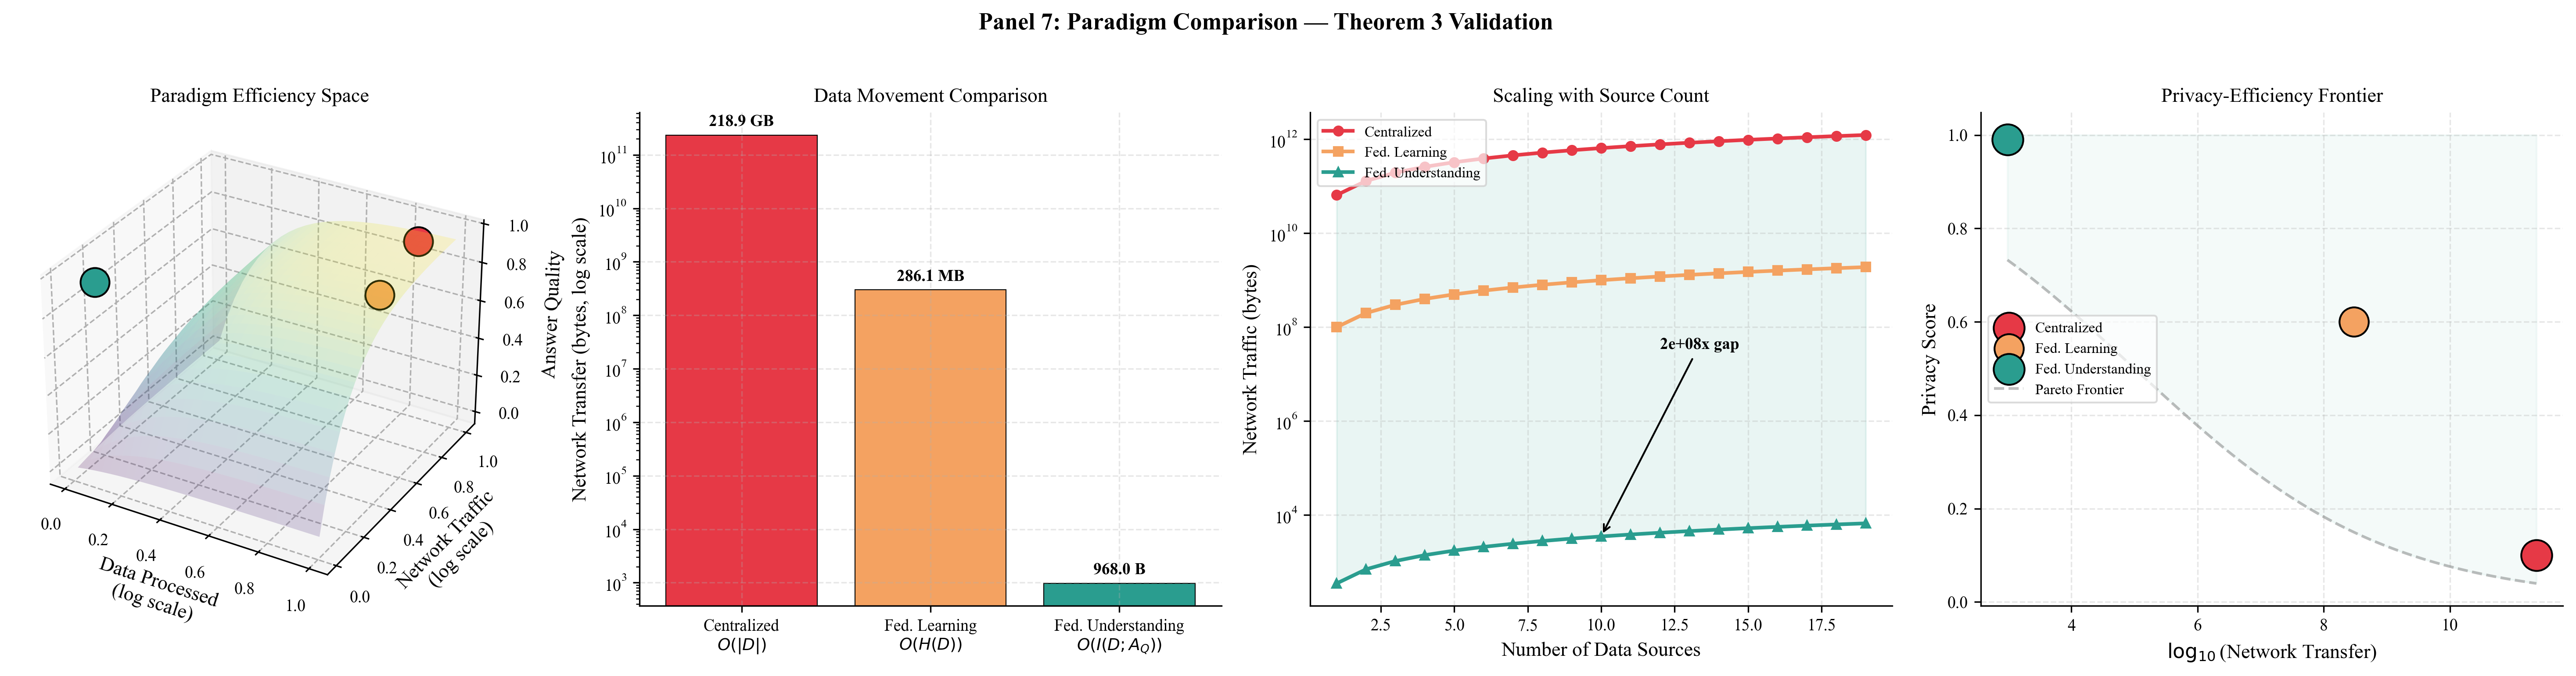
\includegraphics[width=\textwidth]{figures/fed_panel_7_paradigm_advantage.png}
\caption{Paradigm comparison (Theorem~\ref{thm:paradigm_comparison} validation). (a) 3D paradigm efficiency space: data processed vs.\ network traffic vs.\ answer quality. (b) Log-scale network transfer: 218.9~GB (centralized) vs.\ 286.1~MB (federated learning) vs.\ 968~B (federated understanding). (c) Scaling projection: the gap widens to $2 \times 10^{8}\times$ as source count increases. (d) Privacy--efficiency Pareto frontier showing federated understanding at the optimal corner.}
\label{fig:panel7}
\end{figure*}

%==============================================================================
\section{Discussion}
\label{sec:discussion}
%==============================================================================

\subsection{Relation to Existing Paradigms}

\textbf{Federated learning} \cite{mcmahan2017,kairouz2021} trains local models on all local data, then aggregates model parameters. The local model is shaped by the data distribution, not by the research question. Federated understanding inverts this: the question shapes the extraction. Additionally, federated learning aggregation through parameter averaging destroys node-specific structure; understanding composition through categorical intersection preserves it.

\textbf{Retrieval-augmented generation} \cite{lewis2020rag,borgeaud2022} retrieves relevant documents at inference time. This requires maintaining and indexing external knowledge bases, introduces retrieval latency, and limits reasoning to surface-similarity matches between queries and documents. Domain-specific knowledge embedding eliminates retrieval infrastructure while enabling the compositional, contextual, constraint-aware reasoning required for surgical extraction (Theorem~\ref{thm:parametric_necessity}).

\textbf{Multi-agent debate} \cite{du2024} uses multiple language models in adversarial dialogue to improve factuality. The metacognitive pipeline extends this by adding structured decomposition, resource-aware allocation, controlled diversity through determinantal point processes, and formal verification through proof assistants. The pipeline is not a debate but a coordinated investigation with quality gates.

\textbf{Automated scientific discovery} \cite{king2004,kitano2021,wang2023scientific} has focused on hypothesis generation and experimental design. AlphaFold \cite{jumper2021} demonstrated that domain-specific neural architectures can solve longstanding scientific problems. Federated understanding extends this paradigm from single-domain prediction to multi-modal, multi-institution research automation with formal provenance.

\textbf{Self-refinement} \cite{shinn2023reflexion,madaan2023self} enables language models to iteratively improve outputs using self-generated feedback. The metacognitive pipeline incorporates self-refinement as one mechanism (the orchestration stage's \texttt{refine} action) within a broader architecture that includes external validation, multi-expert consensus, and formal verification---mechanisms that cannot be replicated by self-feedback alone.

\subsection{The Research-Question-Shaped Extraction Principle}

The central insight of federated understanding is that the research question determines what information exists in the system. This is not an optimization over conventional pipelines---it is a different computational model. In conventional computation, data exists independently of questions; questions are posed to data. In federated understanding, the question creates the data representation; without a question, no representation exists.

This principle has several consequences:

\textbf{No stale data.} There is no cached representation that can become outdated, because representations are generated on demand from the current question against the current data.

\textbf{No integration step.} Multi-modal integration is traditionally a separate, often bottleneck, stage \cite{picard2021,subramanian2020}. In federated understanding, all modalities map to $\Sspace$ through their observe bridges; integration is composition, which is a built-in categorical operation.

\textbf{No privacy-utility trade-off.} Differential privacy \cite{dwork2006} introduces noise that degrades analytical utility. Structural privacy (Theorem~\ref{thm:privacy}) provides stronger guarantees without any utility cost, because irrelevant data is never processed rather than being processed and then protected.

\textbf{Reproducibility is structural.} The trajectory $T^*$ encodes the complete methodological provenance: every extraction, every composition, every refinement, every validation step. Reproducing the analysis requires only the protocol specification and access to the same (or updated) data sources \cite{wilkinson2016fair}. The analysis is reproducible by construction, not by documentation.

\subsection{Limitations}

\textbf{Domain compiler coverage.} The framework requires domain-specific compilers for each modality. Creating a new compiler requires domain corpus construction, teacher model generation, curriculum design, and student training. This is a significant upfront investment, amortized across all research questions in that domain.

\textbf{Question expressibility.} Not all research questions are expressible in the protocol language. Exploratory research (``what is interesting in this dataset?'') lacks the target specification required for problem-directed extraction. The framework is suited to hypothesis-driven research with clearly defined objectives.

\textbf{Validation depth.} Formal verification is limited to mathematical claims expressible in the proof assistant's logic. Domain-specific validity (``is this biologically plausible?'') relies on domain-expert models, which may themselves be incorrect. The multi-expert consensus mechanism mitigates but does not eliminate this risk.

\textbf{Latent reasoning opacity.} The metacognitive pipeline's reasoning occurs in the latent space of language models. While the trajectory provides structural provenance (what operations were performed), the internal reasoning within each operation is not fully transparent. This is a general limitation of neural network-based systems \cite{brown2020}.

\textbf{Convergence requirements.} The convergence theorem (Theorem~\ref{thm:convergence}) assumes quality-monotonic refinement and sufficient diversity in candidate generation. Pathological question structures or adversarial data distributions may prevent convergence, requiring human intervention through the \texttt{redirect} mechanism.

\subsection{Applications}

The framework is suited to investigations requiring:

\begin{itemize}[nosep]
\item Multi-institutional data access without centralization
\item Multi-omic or multi-modal evidence integration \cite{hasin2017,reel2021}
\item Statistical rigor with formal provenance
\item Privacy-preserving analysis of sensitive data
\item Reproducible methodology specification
\item Automation of expert-level analytical reasoning
\end{itemize}

Candidate domains include clinical research across hospital networks, population-scale genomic studies, pharmacovigilance across regulatory jurisdictions, environmental monitoring across sensor networks, and systematic reviews integrating evidence across publications.

%==============================================================================
\section{Conclusion}
\label{sec:conclusion}
%==============================================================================

We have presented federated understanding: a framework for automated deep research in which the entire scientific analysis process is executed by networks of domain-specific language models coordinated through categorical trajectory completion.

The framework comprises:

\textbf{A research protocol specification language} in which investigations are expressed as trajectory specifications through S-entropy coordinate space. Programs declare what is to be investigated, what evidence is required, and what constitutes a valid conclusion. The system determines how.

\textbf{Problem-directed compilation} in which domain-specific language models translate protocol statements into morphism chains that surgically extract only question-relevant information from distributed data sources. We proved that correctly compiled chains produce sufficient statistics with information content bounded by $I(\dataset; \answer_\question)$ (Theorem~\ref{thm:minimality}).

\textbf{Domain-specific knowledge embedding} in which specialized knowledge is encoded directly into model parameters through knowledge distillation, enabling the compositional, contextual, constraint-aware reasoning required for surgical extraction. We proved that parametric knowledge is necessary; retrieval-augmented approaches are insufficient (Theorem~\ref{thm:parametric_necessity}).

\textbf{Metacognitive refinement} in which a multi-stage optimization pipeline replaces the human researcher's iterative analysis. Question decomposition, information-yield resource allocation, diverse candidate generation through determinantal point processes, multi-dimensional quality evaluation, and quality-gated orchestration produce validated analyses with convergence guarantees (Theorem~\ref{thm:refinement_convergence}).

\textbf{Federated understanding architecture} in which what traverses the distributed network is neither data nor trained models but question-shaped understanding fragments. We proved that network traffic is bounded by $\mathcal{O}(I(\dataset; \answer_\question))$, orders of magnitude less than federated learning's $\mathcal{O}(H(\dataset))$ (Theorem~\ref{thm:paradigm_comparison}), with structural privacy guarantees stronger than differential privacy (Theorem~\ref{thm:privacy}).

\textbf{Multi-expert validation} combining domain-expert consensus, adversarial quality assessment, and formal verification through proof assistants, ensuring that conclusions are correct rather than merely plausible.

\textbf{The analysis graph} whose convergence through variance restoration drives understanding fragments from dispersed gas phase through liquid clustering to crystalline ground state, with the triple completion criterion ensuring categorical convergence, expert validation, and negligible evolution entropy.

The central insight is that the research question determines what information exists in the system. A researcher writes a protocol specification---a precise declaration of what is to be investigated---and receives a validated answer with full trajectory provenance, without manual analysis, without data movement beyond surgical extraction, and without exposing irrelevant information. The path taken through categorical space to reach the answer is the answer's address is the answer's provenance is the answer's proof of methodology.

The framework is falsifiable through: violation of the information minimality bound, failure of composition preservation across modalities, breakdown of convergence under variance restoration, or demonstration that retrieval-augmented compilation achieves equivalent surgical extraction to parametric compilation. These tests provide concrete criteria for empirical evaluation.

Automated deep research is trajectory completion in bounded phase space. The question is the scalpel. Understanding is the currency. The answer crystallizes.

\bibliographystyle{plain}
\bibliography{references}

\end{document}
